
% -*- root: These.tex -*-

\subsection{Une lecture pluri-disciplinaire des problématiques liés à la validation}
\label{ssec:triple_lecture}

%Si le modélisateur est au courant des simplifications opérés dans les hypothèses censés représenter ,  la dynamique de construction introduit dans l'activité de construction des modèles une incertitude supplémentaire qui nous oblige à repenser l'activité de validation.

\subsubsection{Les définitions de la validation en V\&V}
\label{sssec:def_generique_validation}

Les termes \foreignquote{english}{Validation \& Verification} ou \textit{V\&V} proviennent à l'origine de l'ingénierie des systèmes, et peuvent être rattachés au concept de \enquote{qualité} tel qu'il est défini par la famille de règles ISO établies par l'organisation mondiale de normalisation.

Décomposable en plusieurs branches cette discipline à part possède une branche dédiée à l'expertise logicielle. De ce fait, il n'existe pas réellement de définition ni de théories ou méthodologies officiellement acceptables, l'acceptation des termes pouvant varier fortement selon les branches d'application.

On trouve toutefois quelques références dans des livres dédiés à la terminologie standard pour la \enquote{gestion de projet} dans un large panel de disciplines, telle que le PMBOK (\textit{A guide to the project Management Body of Knowledge}) \autocite{PMBOK2013}. Résultats d'un travail certifié par des associations ou des organismes étatiques tels que IEEE et ANSI, ce dernier propose une définition générale de ces termes pour l'ingénierie logicielle :

\foreignquote{english}{Verification and validation (V\&V) processes are used to determine whether the development products of a given activity conform to the requirements of that activity and whether the product satisfies its intended use and user needs.}

et revient ensuite plus spécifiquement sur les termes :

\begin{itemize}
\item \textbf{Validation} \foreignquote{english}{The assurance that a product, service, or system meets the needs of the customer and other identified stakeholders. It often involves acceptance and suitability with external customers. Contrast with verification.}
\item \textbf{Verification} \foreignquote{english}{The evaluation of whether or not a product, service, or system complies with a regulation, requirement, specification, or imposed condition. It is often an internal process. Contrast with validation.}
\end{itemize}

Les termes tels qu'ils sont définis sont finalement bien trop généraux pour envisager de les appliquer tels quels dans notre domaine de compétence. Dérivé de la branche de l'\textit{Operational Research (OR)}, les auteurs de la communauté restreinte des \textit{systems analysis or modelling and Simulation (M\&S) } engagent dès les années 1960-70 des efforts pour standardiser ces définitions pour la simulation.

\Anotecontent{first_time_validation}{La citation de Churchman par \textcite{Naylor1966} est tiré de \autocite[165]{Nance2002} : \foreignquote{english}{\foreignquote{english}{X simulates Y} is true if, and only if, (a) X and Y are formal systems, (b) Y is taken to be the real system, (c) X is taken to be an approximation to the real system and (d) the rules of validity in X are non-error-free.} \autocite{Nance2002} }

Parmi les différents auteurs participant de ce mouvement ( Naylor, Finger, Oren, Hermann, Zeigler, Nance, Banks, Gass, Balci, Sargent, etc.), \textcite{Naylor1966} est considéré avec West Churchman (1963) comme un des tout premier à avoir attiré et cristalisé \Anote{first_time_validation} dans de multiples publications l'attention sur cette problématique importante de la V\&V.

Cet économiste formé à l'informatique dans la branche des \foreignquote{english}{management sciences} \autocite{Stricklin1985} est un des premiers en 1967 \autocite{Naylor1967} à publier dans un article nommé \foreignquote{english}{Verification of Computer simulation models} une méthode abordant spécifiquement la question de la crédibilité des connaissances qui peuvent être apportées par un modèle de simulation. Une méthode qu'il va mettre spontanément en tension avec les débats qui agitent la communauté des philosophes à cette même période.

Malgré ces efforts et sa volonté de porter le débat loin dans la communauté inter-disciplinaire (voir les premiers ouvrage collectifs sur l'usage de la simulation dans les \enquote{behavior science} \autocite{Dutton1971, Guetzkow1972} \hl{A verifier}), la démarcation entre les deux termes est encore peu claire \autocites[165]{Nance2002}[3]{Balci1986}. \footnote{\foreignquote{english}{Thomas Naylor, a coauthor of the book cited above, deserves credit for drawing major attention to the validation issue in the 1960s: Is the model actually representing the truthful behavior of the referent system? His work, above and in later publications (Naylor 1971, Naylor and Finger 1967), exerted a major influence in framing validation within different philosophical perspectives. Numerous techniques that can be used were identified or developed. While the issues of both verification and validation were of concern from the early days of simulation, often no clear distinction was made between the two terms.} \autocite[165]{Nance2002}}

\Anotecontent{balci_standard}{\foreignquote{english}{A uniform, standard terminology is yet nonexistent. A recent literature review \autocite{Balci1984} indicated the usage of 16 terms [...] Except some early papers which appearead between 1966 and 1972, model verification and model validation have been most of the time consistently defined reflecting the following differentiation : \textbf{model verification} refers to building the model right; and \textbf{model validation} refers to building the right model. \autocite{Balci1986}}}

Il faudra attendre le début des années 1980 pour qu'un standard émerge, grâce à des financements étatiques \autocite{Balci1986}, mais également du fait des efforts fournis par des auteurs comme Sargent et Balci \autocite{Nance2002}, qui collectent et organisent dans une typologie cohérente l'existant statistique et méthodologique, une activité qu'ils poursuivent encore aujourd'hui \autocite{Balci1998}.\Anote{balci_standard}

Pour \autocite[22]{Oberkampf2010} \foreignquote{english}{A Key milestone in the early work by the OR community was the publication of the first definitions of V\&V by the Society of Computer Simulation (SCS) in 1979 \autocite{Schlesinger1979}}, un des instituts avec la U.S GAO (U.S General Accounting Office) à fournir des spécifications en 1979 \autocite{Balci1986}

\begin{itemize}
\item \textbf{Model Verification} \foreignquote{english}{substantiation that a computerized model represents a conceptual model within specified limit of accuracy.}
\item \textbf{Model Validation} \foreignquote{english}{substantiation that a computerized model within its domain of applicability possesses a satisfactory range of accuracy consistent with the intended application of the model.}
\end{itemize}

\begin{figure}[h]
\begin{sidecaption}[fortoc]{Un des tout premiers schémas issus de la publication de la SCS \autocite{Oberkampf2010,Schlesinger1979}}[fig:S_VV]
  \centering
 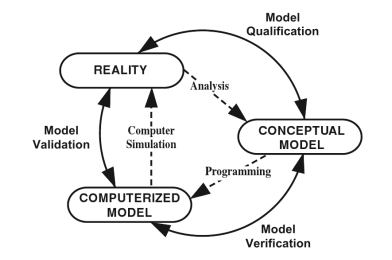
\includegraphics[width=.7\linewidth]{schelinger_schema1979.png}
  \end{sidecaption}
\end{figure}

Même si elles sont plus anciennes et de portée moins générale, ces définitions de la \textit{V\&V} semblent plus pertinentes, car évoquées plus régulièrement par les chercheurs en sciences sociales; les travaux les plus cités étant ceux de \textcite{Kleijnen1995}, ou \textcite{Sargent2010} qui placent leurs travaux dans la continuité de ces définitions. L'avancée de leurs travaux peut être suivie en feuilletant les \textit{Proceedings of the Winter Simulation Conference} où la problématique de la \textit{V\&V} est réévaluée régulièrement au regard des nouvelles connaissances. Ce schéma \ref{fig:S_VV} est devenu un classique repris et régulièrement amendé \autocite{Sargent2010}. Voici la lecture qu'en fournit \autocite{Oberkampf2010}

\foreignquote{english}{The \textbf{conceptual model} comprises all relevant information, modelling assumptions, and mathematical equations that describe the physical process or process of interest. [...] The SCS defined \textbf{qualification} as \enquote{Determination of adequacy of the conceptual model to provide an acceptable level of agreement for the domain of intended application}. The \textbf{computerized model} is an operational computer program that implements a conceptual model using computer programming. Modern terminology typically refers to the computerized model as the computer model or code.}

Ce schéma a la particularité suivante, il \foreignquote{english}{ [...] emphasizes that \textbf{verification} deals with the relationship between the conceptual model and computerized model and that \textbf{validation} deals with the relationship between the computerized model and reality. These relationships are not always recognized in other definitions of V\&V [...]}

\Anotecontent{Kleijnen_def}{\foreignquote{english}{This paper uses the definitions of V \& V given in the classic simulation textbook by Law and Kelton (1991, p.299): \enquote{Verification\textbf{Verification} is determining that a simulation computer program performs as intended, i.e., debugging the computer program .... \textbf{Validation} is concerned with determining whether the conceptual simulation model (as opposed to the computer program) is an accurate representation of the system under study}. Therefore this paper assumes that verification aims at a \enquote{perfect} computer program, in the sense that the computer code has no programming errors left (it may be made more efficient and more user friendly). Validation, however, can not be assumed to result in a perfect model, since the perfect model would be the real system itself (by definition, any model is a simplification of reality). The model should be \enquote{good enough}, which depends on the goal of the model.}}

\Anotecontent{Sargent_def}{\foreignquote{english}{\textbf{Model verification} is often defined as \enquote{ensuring that the computer program of the computerized model and its implementation are correct} and is the definition adopted here. \textbf{Model validation} is usually defined to mean \enquote{substantiation that a computerized model within its domain of applicability possesses a satisfactory range of accuracy consistent with the intended application of the model} \autocite{Schlesinger1979} and is the definition used here. A model sometimes becomes accredited through model accreditation. Model accreditation determines if a model satisfies specified model accreditation criteria according to a specified process. A related topic is model credibility. Model credibility is concerned with developing in (potential) users the confidence they require in order to use a model and in the information derived from that model. A model should be developed for a specific purpose (or application) and its validity determined with respect to that purpose [...]A model is considered valid for a set of experimental conditions if the model’s accuracy is within its acceptable range, which is the amount of accuracy required for the model’s intended purpose.}}

Autrement dit, \foreignquote{english}{The OR community clearly recognized, as it still does today, that V\&V are tools for assessing the accuracy of the conceptual and computerized models.} Un avis partagé par \textcite{Kleijnen1995} \Anote{Kleijnen_def} , \textcite{Balci1998}, et \textcite{Sargent2010} \Anote{Sargent_def} mais également des auteurs de références sur le sujet dans les sciences humaines et sociales \autocite{Amblard2006} \hl{Prend le bout de texte la dessus}.

Seulement, cette forme de relâchement sur la correspondance entre réalité et modèle, et ce positionnement plus relativiste de la validation n'a pas toujours été une évidence; les premières définitions de Naylor par exemple, sont toujours usitées, et continuent si on en croit des auteurs comme \textcite{Kleindorfer1998} à semer le trouble dans certaines disciplines.

\Anotecontent{VV_philout}{ \foreignquote{english}{During the last two decades a workable and constructive approach to the concepts, terminology, and methodology of V\&V has been developped, but it was based on pratical realities in business and government, \textbf{not} the issue of obsolute thruth in the philosophy of nature} \autocite{Oberkampf2010}
\foreignquote{english}{A very old philosophical question is: do humans have accurate knowledge of reality or do they have only flickering images of reality, as Plato stated? In this paper, however, we take the view that managers act as if their knowledge of reality were sufficient. Also see Barlas and Carpenter (1990), Landry and Oral (1993), and Naylor, Balintfy, Burdick and Chu (1966, pp.310-320).} \autocite{Kleijnen1995}
\foreignquote{english}{With the strong interest in verification from the software engineering community, this contrasting but complementary explanation of the term was quite important. The effort to place valida- tion in a cost-risk framework moved the concept from a philosophical explanation in earlier works to a form more useable for simulation practitioners.} \autocite[165-166]{Nance2002}}

Mais en excluant ainsi de son analyse la partie subjective et philosophique de la \enquote{Validation}\Anote{VV_philout} pour se concentrer sur la seule partie opérationnelle, ces méthodologies restent pour le modélisateur une coquille vide décevante, qui demande encore à être incarnée thématiquement. Autrement dit, ces méthodes si elles prennent bien en compte la dimension dynamique et incrémentale nécessaire à la construction d'un modèle de simulation qui tendrait vers une réalité en accord avec la question posée, l'organisation des connaissances nécessaires pour guider ce processus reste à la lecture de ces typologies une opération quelque peu énigmatique pour les modélisateurs géographes. On retombe sur une des critiques soulevées précédemment dans la section \ref{sec:critiques_simulation} sur l'absence constatée dans les publications de méthodologie standard pour la validation qui prendrait en compte les problématiques spécifiques d'une discipline. \footnote{Aujourd'hui des disciplines comme l'écologie proposent des méthodologies plus spécifiques, comme la méthode POM proposé par Grimm sur lequel nous reviendront par la suite \hl{mettre une ref et un appel à la section}}

Une position compréhensible pour ces auteurs oeuvrant pour la standardisation, alors même que ces termes sont toujours d'usages toujours assez variables. Une des conséquences visibles tient dans ces incompréhensions et ces débats terminologiques sans fin \autocite{David2009} que l'on observe parfois en marge des discussions inter-disciplinaires. Cette gamme d'acceptions différentes tient souvent au transfert hasardeux des terminologies entre l'ingénierie des M\&S, la philosophie des sciences, et la thématique d'un chercheur en sciences sociales qui se retrouve en position intermédiaire de ces deux derniers. Un exercice d'équilibriste périlleux, car comme le fait remarquer \textcite{Kleijnen1995} en citant astucieusement une note de bas de page de \textcite{Barlas1990}, en philosophie il est tout à fait possible de voir la signification des deux termes inversée! \hl{Expliquez mieux que verification pourrait se traduire en philosophie pour certains par representation de la vérité, du “reel”, alors que le fait même de modéliser implique qu’on en soit loin}

\subsubsection{La philosophie des sciences}

Il ne s'agit pas de se lancer ici dans un exposé historique des courants et débats s'étant succédés dans cette discipline, mais d'amener de façon illustrative et avec quelques références récentes l'émergence ces 20 dernières années d'une \enquote{épistémologie de la simulation} reprenant (en parasitant parfois le débat comme on l'a cité au dessus) de son point de vue certains débats évoqués chez les praticiens de la simulation; la question de validation étant comme on l'a vu dans le chapitre 1 un sujet de longue date chez les praticiens de la simulation, mais aussi chez les premiers acteurs fondateurs de la V\&V.

\hl{redite : L'objectif n'est donc pas tant de développer une argumentation critique exposant l'ensemble de ces points de vues, car ce n'est pas l'objet de cette thèse, que de tenter de s'insérer (et non de s'enfermer) dans ces réflexions en spécifiant en quoi celle ci diffère, néglige ou font peu écho à nos pratiques et réflexion historique en sciences sociales.}

Le premier obstacle avec laquelle les acteurs supportant cette nouvelle épistémologie doivent cohabités est évidemment la contre-argumentation questionnant cette même necessité d'opérer une nouvelle sous-division épistémologique. Car existe-t-il réellement des spécificité à la connaissance dérivé de l'étude de l'objet simulation, et si oui quelles sont elles réellement ? Autrement dit, existe t il une différence fondamentale entre les questionnements déjà posés dans le cadre d'une épistémologie des modèles et ceux évoqués dans le cadre d'une épistémologie de la simulation ?

\Anotecontent{frilosite_philoScience}{\foreignquote{english}{As computer simulation methods have made their way into novel disciplines, the issue of their trustworthiness for generating new knowledge has often loomed large, especially when they have competed for attention with experiments or analytically tractable modeling methods. The relevant question is always whether or not the results of a particular computer simulation are accurate enough for their intended purpose.[...] Given our long-standing preoccupation with issues of confirmation, it might seem obvious that philosophers of science would have the resources to easily approach these questions.} \autocite{Winsberg2013}}

Parmis les auteurs ouvertement favorable à la création d'une nouvelle épistémologie, on citera entre autre les efforts de \autocites{Winsberg2001, Winsberg2009, Winsberg2013} qui pousse dans chacune de ses publications les \enquote{philosophes des sciences} à sortir de la seule étude de la \enquote{théorie de la confirmation} pour aller vers un terrain un peu plus aventureux \Anote{frilosite_philoScience}, celui de l'étude de la crédibilité des explications et des hypothèses dans leur dépendance au contexte.

Il propose de résumer l'originalité d'une telle épistémologie en évoquant l'inférence spécifique que produisent l'étude simultanée de trois point sur la simulation. \foreignquote{english}{ \textcite{Winsberg2001} argued that, unlike the epistemological issues that take center stage in traditional confirmation theory, an adequate EOCS must meet three conditions. 
downward, motley, and autonomous.[...] These three features were meant to be offered as conditions of adequacy; for which any adequate epistemology of simulation must account. Against the background of the growing use of simulation in the sciences, an adequate epistemology for the philosophy of science needs to explain the fact that simulation results and computational models are often taken to be reliable despite these three features. Winsberg (2001) argues that simulation requires a new epistemology precisely because traditional stories in philosophy of science about how knowledge claims get credentialed cannot explain them.}

Cette typologie a soulevé un certain nombre de critiques chez les philosophes des sciences, dont la plus longue et la plus argumenté est surement celle de \textcite{Frigg2009} dont on trouve le résumé des points saillants dans les publications de \textcites{Winsberg2009, Winsberg2013} mais également de bien d'autres auteurs qui se réfèrent à ce débat pour se positionner \textcites{Yanoff2010, Eckhart2010}.

Le deuxième point de débat intéressant réside dans le qualificatif souvent donné à la simulation de \enquote{laboratoire virtuel pour l'expérimentation}. Si les philosophes des sciences ne peuvent que s'incliner face au constat d'une telle banalisation du terme, dont nous avons donné nous même un aperçu de son ancienneté d'usage dans les sciences sociales dans le chapitre 1; il existe quand même chez les philosophes la volonté de mettre à l'épreuve les fondements et les conséquences pour la connaissance extraite d'une telle analogie.

\Anotecontent{HackingCartwright}{\enquote{Nos deux livres ont plus d'un point commun. L'un et l'autre accordent peu d'importance à la vérité des théories et avouent un faible pour certaines entités théoriques. Cartwright soutient que seules les lois phénoménologiques de la physique parviennent à la vérité tandis que, dans la partie B de ce livre, je fais remarquer que la science expérimentale est plus indépendante de la théorie que ce que l'on veut bien généralement admettre. Nous ne partons pas des mêmes postulats anti-théoriques car elle considère les modèles et les approximations alors que c'est surtout l'expérience qui m'intéresse, mais nos conceptions convergent.}\autocite{Hacking1983}}

\Anotecontent{Phan_Varenne_theorie}{\foreignquote{english}{Consequently, in the first neo-positivist epistemology, models were viewed not as autonomous objects, but as theoretically driven derivative instruments. Following the modelistic turn in mathematical logic, the semantic epistemological conception of scientific models persisted to emphasize on theory.} \autocite{Phan2010}}

Un débat d'autant plus actif qu'on assiste depuis ces 20 dernières années à un véritable renouveau des questionnements dans le cadre d'une \enquote{épistémologie de l'expérimentation} jusqu'alors relativement peu considéré par la majorité des philosophes des sciences \Anote{Phan_Varenne_theorie}. \textcites{Phan2008, Phan2010} citent ainsi les contributions importantes d'auteurs comme Fischer(1996), Galison (1987, 1997), Franklin (1986, 1996), Morrisson(1993, 1999), mais également les efforts de Hacking (1983) et Cartwright.

\Anotecontent{def_cartwright}{\enquote{Disons qu'il y a des théories, des modèles et des phénomènes. Il serait normal de penser que les modèles sont doublement des modèles. Ils sont modèles pour les phénomènes et modèles pour la théorie. [...] Le réalisme scientifique est ici tout particulièrement concerné. Cartwright est pour l'essentiel anti-réaliste à propos des théories. Pour cela, elle s'appuie en partie sur les modèles. Elle fait remarquer que non seulement les modèles ne peuvent être déduits de la théorie qui les englobe, mais plus encore que les physiciens utilisent à leur gré divers modèles qui, sans pourtant se recouper, cohabitent tous au sein de la même théorie. Et cependant,ces modèles sont les seules représentations formelles disponibles des lois phénoménologiques que nous tenons pour vraies. Elle affirme que seules ces lois phénoménologiques nous permettent d'avancer. Toutes les modélisations de ces lois ne peuvent être vraies ensemble puisqu'elles ne sont pas compatibles. Et rien ne permet de penser qu'un modèle est supérieur à un autre. Aucun n'est vraiment justifié par la théorie qui le porte. Plus encore, les modèles ont tendance à résister aux changements de théorie, c'est-à-dire que le modèle est conservé même si la théorie s'avère inadéquate. Il y a plus de vérité locale dans les modèles incompatibles que dans les théories, pourtant plus sophistiquées.[...] L'idéal de la science n'est pas l'unité mais dans une abondance et diversité de plus en plus grandes.} \autocite[350]{Hacking1983}}

\Anotecontent{def_hacking}{\enquote{Le \textit{réaliste à propos des entités} affirme que bon nombre d'entités théoriques existent vraiment. L'anti-réaliste s'oppose à ces entités qui ne sont pour lui que fictions, constructions logiques ou éléments d'un processus intellectuel d'appréhension du monde. Un anti-réaliste moins dogmatique dirait que nous n'avons pas, et ne pouvons avoir, de raison de supposer que ces entités ne sont pas des fictions. Peut-être existent-elles,mais le présupposer n'est pas nécessaire à notre compréhension du monde. 

Le \textit{réaliste à propos des théories} dit que les théories
sont soit vraies, soit fausses et ce indépendamment de ce que nous percevons : la science, elle au moins, vise à obtenir la vérité et la vérité est le monde tel qu'il est. L'anti-réaliste dit des théories qu'elles sont au mieux
prouvées, adéquates, opératoires, acceptables - quoi-que incroyables, entre autres qualificatifs possibles. } \autocite[59]{Hacking1983}}

On retiendra principalement pour notre argumentaire cette propriété d'indépendance retrouvé de l'expérimentation par rapport à la théorie \Anote{def_cartwright}, dont on peut trouver un très bon manifeste dans les écrits de \textcite{Hacking1983} et Cartwright \Anote{def_hacking}, ces derniers se positionnant comme des antiréalistes des théories, tout en étant des réalistes des entités théoriques. Un point de vue très bien résumé à la fois dans \textcite{Hacking1983} et \textit{Théorie, Réalité, Modèle} de \textcite[226-231]{Varenne2012}

Sur la notion de modèle dans sa relation à l'expérimentation, il semblerait qu'un consensus se dégage chez les philosophes \autocites{Morgan2009, Varenne2013} autour du modèle perçu comme un \enquote{médiateur autonome} articulant théorie, pratiques et données dans un contexte spécifique d'une question et d'un cadre technico-social. \autocite[2]{Phan2010}

Il y a probablement un point intéressant à développer entre cette argument du modèle autonome, et les récents travaux en sciences sociales pour qualifier au travers d'une grille de lecture \autocites{Banos2013a, Sanders2013} le positionnement \autocites{Banos2013, Schmitt2013} et le déplacement des modèles de simulation au travers d'une part de leur construction \autocite{Cottineau2014b}, mais également de leur réutilisation \autocite{Schmitt2014}. Une autre façon de démontrer en quoi cette capacité à cumuler de façon flou différentes fonctions épistémiques donné dans la spécification minimale de Varenne pour la simulation \autocite{Varenne2013} est intéressante dès lors qu'il s'agit de tracer la trajectoire disciplino-temporelle de certains modèles : daisyWorld \autocite{Dutreuil2013}, Schelling \autocite {Bulle2005}, SugarScape, etc.)

\Anotecontent{winsberg_exper_simu_link}{Another unique feature of the epistemology of simulation is the ease with which it can draw inspiration from the epistemology of experiment.}

Les acteurs pronant comme Winsberg une épistémologie de la simulation n'hésite alors pas à débattre pour ce qui est des différents parallèle que l'on peut tracer avec les réflexions de cette communauté. \Anote{winsberg_exper_simu_link}.

Pour ne pas se perdre dans les différents points de vues sur le sujet et bénéficier d'une vue plus large incluant les réflexions des praticiens, on pourra se référer au travail opéré par \textcite{Varenne2001} dans son article \textit{What does a computer simulation prove?}, qui propose une lecture du débat au travers de d'une typologie soulevant trois grandes thèses : I - La simulation est elle un outils commes les autres \textit{A simulation is only a tool} ? II - ou bien l'équivalent fusionnel d'une expérimentation classique (\textit{A simulation is an experiment}) ? III - ou se positionne-t-elle comme médiateur entre la théorie et expérimentation ? (\textit{A computer simulation is an intermediate between theory and experiment})? 

%L'expérimentation mène sa vie propre et entretient diverses relations avec la spéculation, le calcul, la construction de modèles, l'invention et la technologie. Mais alors que le calculateur, le spéculateur et le constructeur e modèles peuvent être anti-réalistes, l'expérimentateur, lui, doit être réaliste. p18 

On trouve donc un grand nombres de travaux, toutes disciplines confondues (les philosophes des sciences ne sont pas les seuls à se poser ce type de question, comme nous verrons par la suite), qui tentent d'établir par le biais de différentes grilles de lecture l'appartenance de ce \enquote{nouveau?} mode d'expérimentation à une des catégories de cette grille. \textit{Pourquoi ? Au delà du jeu d'esprit, quel est l'enjeu motivant une telle comparaison ?}

\Anotecontent{moto_hacking}{Une remarque qui renvoie d'ailleur explicitement à sa lecture du moto d'Hacking \foreignquote{english}{experiments have a life of their own} et à la notion d'autonomie (\textit{autonomous}) de sa synthèse précédemment, qui marque le fait que dans certains cas (impossibilité d'observation, manque de données), la simulation doit faire la preuve des connaissances (\textit{background knowledge}) apportés sur appel de ses propres ressources.}

\Anotecontent{experimental_warranting_belief}{\foreignquote{english}{The central idea of this thread is that experiments are the canonical entities that play a central role in warranting our belief in scientific hypotheses, and that therefore the degree to which we ought to think that simulations can also play a role in warranting such beliefs depends on the extent to which they can be identified as a kind of experiment} \autocite{Winsberg2009}}

Partant du fait que l'expérimentation joue un grand rôle dans l'établissement d'une crédibilité pour les hypothèses avancés, il s'agit de mesurer à quel point la simulation serait susceptible d'apporter les mêmes garanties dès lors qu'on accepte de la voir comme une sorte d'expérimentation.\Anote{experimental_warranting_belief}

On s'appuiera dans la suite de cette argumentation sur la lecture de Winsberg, un philosophe des sciences que l'on estime plutôt partisan de la III thèse dans la classification ci dessus. Ce dernier s'appuie largement sur les travaux d'Hacking, mais aussi Galison pour construire sa réflexion, par exemple en arguant\foreignquote{english}{ [...] that some of the techniques that simulationists use to construct their models get credentialed in much the same way that Hacking says that instruments and experimental procedures and methods do; the credentials develop over an extended period of time and become deeply tradition-bound.} \autocites{Winsberg2003, Winsberg2013} \Anote{moto_hacking}

Winsberg résume ce débat en deux thèses opposés : \foreignquote{english}{Identity Thesis} qui consiste à dire que la simulation est littéralement une expérimentation, et \foreignquote{english}{Epistemology Identity Thesis} qui consiste à penser qu'il existe une dépendance entre les garanties de crédibilité qui pourront être accordé par les résultats de la simulation et leur capacité à être plus ou moins définie en tant qu'expérience. Si la première thèse semble assez bien correspondre au point I de la classification de Varenne, la deuxième semble être une sous-variation du point I.

La plupart des auteurs cités par la suite dans ce débat sont des philosophes des sciences spécialisé en économie (Guala , Morgan, Maki, Simon ) qui rejettent comme Winsberg (plus spécialisé en physique) assez naturellement ces deux thèse \autocite{Winsberg2009}, mais avec des arguments assez différents, qu'il convient d'évoquer pour bien comprendre la complexité de ce débat, assez théorique. 

\Anotecontent{maki_phan}{\foreignquote{english}{For Mäki, abstractions in models are similar to abstractions in experiments as they both can be interpreted as a kind of isolation [...] This analogy between models and experiments is called \enquote{isolative analogy} by Guala (2008). From Mäki’s standpoint, a model can be said to be experimented in its explanatory dimension: the finality of such a model is to explore the explanatory power of some causal mechanism taken in isolation.} \autocite{Phan2008}}

Parmis les différents point de vue existant, on citera par exemple le sous-débat de l'\foreignquote{english}{isolative analogy} relaté ici au travers des publications de \textcite{Phan2008, Phan2010} apellant les points de vue de Morgan et Guala contre Maki (2005). Ce dernier voit dans la similitudes entre isolement théorique du modèle comme expérience de pensée et isolement expérimental \Anote{maki_phan} la possibilité de rejoindre une des deux thèses évoqués par Winsberg, établissant d'une façon ou d'une autre que \textit{les modèles sont des expériences, et les expériences des modèles}. Mais ce type d'argument, et on le suppose tout ceux qui se rapportent à l'évocation d'analogies pour justifier d'une équivalence de puissance épistémique se heurterai, comme on va le voir, à une différence fondamentale.

\Anotecontent{guala_phan_winsberg}{Winsberg résume le point de vue de Guala(2002) ainsi \foreignquote{english}{Guala argues that simulation differ fundamentally from experiments in that the object of manipulation in an experiment bears a material similarity to the target of interest, but in a simulation, the similarity between object and target are merely formal.}, mais on peut trouver une version réactualisé en 2008 dans l'article de \textcite[4.2]{Phan2010} \foreignquote{english}{In a simulation, one reproduces the behavior of a certain entity or system by means of a mechanism and/or material that is radically different in kind from that of a simulated entity (...) In this sense, \enquote{models simulate} whereas \enquote{ experimental systems} do not. Theoretical models are conceptual entities, whereas experiments are made of the same \enquote{stuff} as the target entity they are exploring and aiming at understanding}\autocite[14]{Guala2008}}

\textcite{Phan2010} et \textcite{Winsberg2013} cite le point de vue de Guala (2002, 2008), partagé par Morgan(2002, 2005) et se référant aux travaux de Simon (1969). Ceux-ci s'appuient sur une différence de relation qui existe entre système à étudier et système cible dans chacun des deux cas. En effet, dans le cas des expérience, la comparaison s'appuie avant tout sur une similarité matérielle, alors que dans le cas de la simulation la comparaison est limité à une comparaison formelle entre les objets.\Anote{guala_phan_winsberg}

\Anotecontent{Winsberg_critique_morvan}{\foreignquote{english}{Interestingly, while Morgan accepts this argument against the identity thesis, she seems to hold to a version of the epistemological dependency thesis. She argues, in other words, that the difference between experiments and simulations identified by Guala implies that simulations are epistemologically inferior to real experiments - that they have intrinsically less power to warrant belief in hypotheses about the real world.} \autocite[841]{Winsberg2013}}

Morgan(2002, 2005) accepte le point de vue Guala et Simon, mais s'en sert pour réduire indirectement le pouvoir épistémique de la simulation. Un argument bien résumé par \textcite{Phan2008} \enquote{Pour Morgan (2005) modèles et expériences partagent des fonctions de médiateurs et peuvent fonctionner \textit{sur un mode expérimental}, mais les expériences \textit{réelles} offrent un \textit{pouvoir épistémique} d'investigation de la réalité empirique plus fort.} Ce qui fait dire à Winsberg que Morgan serait indirectement plutot partisan de sa deuxième thèse.\Anote{Winsberg_critique_morvan}
\Anotecontent{winsberg_mereformal}{\hl{A compléter avec ce que dit Winsberg2013}}

Pour \textcite{Winsberg2009} le flou des arguments avancé par Morgan et Guala  (\textit{material similarity}, \textit{mere formal similarity}) ne permet pas d'exclure complétement et définitivement la première thèse.\Anote{winsberg_mereformal} Celui-ci se range malgré tout du coté de Guala, et préfère là aussi rejetter cette thèse, mais à la faveur de sa propre argumentation; ce qui lui permet de rejetter à la fois l'argument Morgan pointant l'infériorité épistémique de la simulation, et la deuxième thèse. Il argue que les simulations et l'expérience diffère principalement par la nature du \textit{background knownledge}, c'est à dire protocoles et les connaissances mobilisés.

Des modélisateurs et épistémologues en sciences sociales beaucoup plus proche de nos pratique comme Phan et Varenne trouve un argument convaincant dans ce dernier point, car \foreignquote{english}{Aujourd'hui, comme le souligne Winsberg, la crédibilité des modèles de simulation repose largement sur la \textit{confiance} que nous pouvons avoir dans les compétences des modélisateurs, informaticiens, expérimentateurs et observateurs, ainsi que dans les composants ou plateformes qui supportent les expériences de simulation.} \textcite{Phan2008}

\Anotecontent{gilbert_critique}{\foreignquote{english}{\enquote{[t]he major difference is that while in an experiment, one is controlling the actual object of interest (for example, in a chemistry experiment, the chemicals under investigation), in a simulation one is experimenting with a model rather than the phenomenon itself.} \autocite[14]{Gilbert2005}. But this doesn't seem right. [...] It is false that real experiments always manipulate exactly their targets of interest. In fact, in both real experiments and simulations, there is a complex relationship between what is manipulated in the investigation on the one hand, and the real-world systems that are the targets of the investigation on the other. In cases of both experiment and simulation, therefore, it takes an argument of some substance to establish the ‘external validity’ of the investigation – to establish that what is learned about the system being manipulated is applicable to the system of interest. Mendel, for example, manipulated pea plants, but he was interested in learning about the phenomenon of heritability generally \autocite{Winsberg2013}}}

\Anotecontent{guala_morgan_reality_experiments}{\foreignquote{english}{The identity thesis itself has drawn criticism from Guala (2002) and Morgan(2002). Guala begins by dismissing what he takes to be a poor argument against it. The poor argument goes something like this : simulations are not at all like real experiments because real experiments manipulate the real-world systems that are the very target of the investigation, while simulation merely manipulate \enquote{models} of the target system. What both Guala and Morgan correclty point out is that it is, quite generally speaking, false.}}

Autre sous-débat évoqués par \textcite{Winsberg2013}, on suppose en partie en réponse à sur son article précédent et très similaire \autocite{Winsberg2009}, la critique de l'\textit{identity thesis} comme évoqué par Gilbert et Troitzsch (1999), dont il pense \Anote{gilbert_critique}, en accord avec Guala (2002) \autocite{Winsberg2009} mais également Morgan et Parker \autocite{Winsberg2013} qu'elle est un argument trop faible pour rejeter l'\textit{identity thesis}. \Anote{guala_morgan_reality_experiments} 

Si les arguments de Winsberg semblent convaincant, \textcites{Peschard2010b, Peschard2013} tente dans une analyse critique d'en montrer les biais, et apporte dans son article des objections tout à fait crédible issue de son domaine d'expertise. Pour ne citer qu'un de ces argument, si il existe bien un intermédiaire de mesure issue d'un modèle, comme l'indique Winsberg, il existe également un sous système en prise directe avec la réalité physique de ce monde. En conclusion, elle estime que si il y a bien une certaine forme de similarité entre cibles épistémiques de la simulation et de l'expérience, pour elle ces activités ne peuvent pas être épistémiquement équivalentes, ce qui n'empeche en rien selon elle la coopération fructeuse des deux approches. \hl{Ajouter une footnote avec explication}

\textcite{Winsberg2013} résume le point de vue de \autocite{Peschard2010} ainsi, \textit{Thus, simulation is distinct from experiment, according to her, in that its epistemic target (as opposed to merely its epistemic motivation) is distinct from the object being manipulated.} Autrement dit, même si la motivation menant à l'expérience est bien eloigné (la motivation), l'objet manipulé dans une expérience est bien celui du monde physique, alors que dans le cas de la simulation c'est l'ordinateur. Or autant la motivation peut apprendre de l'objet manipulé dans le monde physique, autant il n'est pas ici dans notre intérêt d'apprendre sur l'ordinateur en tant qu'objet. Dans ce cas là on pointe une différence, mais on peut également appeler selon \textcite{Winsberg2013} et Morrisson (2009) l'argument inverse pointant au contraire une similarité. L'objet expérimenté étant le plus souvent choisi en tenant compte justement de sa capacité de \textit{surrogate} rapport à la question que l'on se pose effectivement, un point commun entre la construction de simulation et d'expérimentation. 

Winsberg conclu en ajoutant que l'expérimentation, contrairement à ce que l'on pourrait penser, n'est pas forcément et immédiatement plus crédible si on ne lui ajoute pas un bagage de connaissance : \textit{Experiments are not automatically more reliable than simulations, despite their differences. [...] It would seem that there are identifiable differences between ordinary experiments and simulations, but there is nothing about these differences that makes one or the other intrinsically more epistemically powerful.}  \autocites{Winsberg2009, Winsberg2013}

\textcite{Varenne2001} avance alors un autre argument intéressant : \foreignquote{english}{Indeed, when you read (Von Neumann 1951), you see that analog models are inferior to digital models because of the accuracy control limitations in the first ones. Following this argument, if you consider a prototype, or a real experiment in natural sciences, is it anything else than an analog model of itself? The test on the prototype is a real experiment. But is it something different and better than the handling of an analog model? So the possibilities to make sophisticated and accurate measures on this model - i.e. to make sophisticated real experiment - rapidly are decreasing, while your knowledge is increasing. These considerations are troublesome because it sounds as if nature was not a good model of itself and had to be replaced and simulated to be properly questioned and tested! It looks as if it was not possible any more to end a paper on simulation by reassuringly using the traditional word: \enquote{Simulation will never replace real experiments”.} }

Ces derniers paragraphes montrent que le débat est loin d'être fixé, et il semblerait là encore que ce soit la définition du contexte d'application qui détermine le mieux la capacité explicative de la simulation, car comme le dit Winsberg \enquote{l'impossibilité d'expérimenter} existe dans bien des disciplines, comme les sciences sociales, mais également la biologie ou la physique, ou les tentatives de reconstitution simulé d'univers ou d'étoiles dans des super calculateur de plus en plus puissant montre qu'il existe un interet explicatif à cette pratique. On pensera notamment aux projets d'expérimentation récents extremement complexe et couteux en physique (laser megajoule de bordeaux, projet ITER pour la fusion).

Et c'est sur ce point que l'argumentation de la plupart des philosophes des sciences est tout à la fois aussi intéressant que problématique. Pour continuer sur Winsberg, celui ci traite de ces problématiques en se positionnant uniquement du point de vue des sciences physiques. Un fait dont il reconnait prudement les conséquences que peuvent avoir l'inclusion d'un contexte différent sur sa synthèse : \foreignquote{english}{Parker (forthcoming) has made the point that the usefulness of these conditions is somewhat compromised by the fact that it is overly focused on simulation in the physical sciences, and other disciplines where simulation is theory-driven and equation-based. This seems correct. In the social and behavioral sciences, and other disciplines where agent-based simulation (see 2.2) are more the norm, and where models are built in the absence of established and quantitative theories, EOCS probably ought to be characterized in other terms.

For instance, some social scientists who use agent-based simulation pursue a methodology in which social phenomena (for example an observed pattern like segregation) are explained, or accounted for, by generating similar looking phenomena in their simulations (Epstein and Axtell 1996; Epstein 1999). But this raises its own sorts of epistemological questions. What exactly has been
accomplished, what kind of knowledge has been acquired, when an observed
social phenomenon is more or less reproduced by an agent-based simulation?
Does this count as an explanation of the phenomenon? A possible explanation?
(see e.g., Grüne-Yanoff 2007).

It is also fair to say, as Parker does (forthcoming), that the conditions outlined above pay insufficient attention to the various and differing purposes for which simulations are used (as discussed in 2.4). [...] Indeed, it is also fair to say that much more work could be done in classifying the kinds of purposes to which computer simulations are put and the constraints those purposes place on the structure of their epistemology.}

Des philosophes des sciences ont donc saisi cette opportunité de critiquer l'approche de Winsberg pour soulever dans des tentatives de typologies parfois intéressantes \autocite{Eckhart2010} les points de divergences que soulève l'utilisation d'une philosophies des sciences naturelle inadapté à la simulation en sciences sociales. Malheureusement, au cours de ces mêmes lectures, on constate que cette critique se retourne vers les modélisateurs et praticiens des sciences sociales, et mène cette fois ci dans une analyse incomplète du contexte historique au mieux à des interprétations erronés (voir le débat animé entre \autocite{Yanoff2008}  \autocites{Elsenbroich2012, Chattoe2011}), et au pire à des approximations et  conseils de mise en oeuvre totalement déplacé \autocite{Eckhart2010} vis à vis de disciplines qui disposent comme on l'a vu d'une véritable histoire autour de l'usage des méthodes computationelles.

Car bien que la recherche des points communs et des différences entre réalité de l'expérimentation physique et virtuelle apparaisse comme un débat intéressant, il faut bien avouer que celui ci ne peut que difficilement s'adapter à la quasi absence d'expérimentation au sens classique dans les sciences sociales. Ainsi, même si la simulation partage certaines des propriétés de l'expérimentation classique, il y a quand même quelque chose de paradoxal à vouloir absolument analyser le rapport de la simulation à l'expérimentation alors même que c'est cette absence qui justement motive son utilisation dans notre discipline, hormis peut etre pour mettre plus en avant cette incapacité à formuler un unique cadre fédérateur par un tel débat. Comme le dit très justement \textcite{Phan2008} {[...] les sciences économiques et sociales sont plus volontiers concernées par l’opposition entre \enquote{le modèle et l’enquête}  (Gérard-Varet et Passeron, 1995) que par celle entre \enquote{l’expérience et le modèle} (Legay, 1997)}

La notion de modèle vue comme médiateur autonome entre théorie et modèle doit elle aussi être repensé pour les sciences humaine, et la géographie; car les théories si elles peuvent exceptionnelement servir à dériver des modèles, celle ci ne peuvent qu'être difficilement rapporté à leur équivalent en science physique \autocite{Pumain1997}.

D'un coté les sciences physiques semble encore viser l'etablissement d'un cadre fédérateur alors qu'il semble que les théories et les modèles en sciences sociales - hormis peut être le cas particulier de l'économie - soit au contraire pourvoyeur de richesse dans leur capacité à apporter un nouvel éclairage sur un phénomène observé. \hl{a préciser peut etre}

A cela il faut ajouter que le modèle en géographie opère dans un cadre épistémique particulier qui n'est pas forcément celui de toute les sciences humaines. Ainsi, bien que les notions et le rapport entre les notions d'observation du \textit{singulier} et du \textit{général} soient théoriquement à la portée de toute disciplines \autocite{Dastes1992}, il semblerait que la géographie trouve un intérét particulier pour la constitution de sa démarche explicative à articuler des éléments de connaissance pris dans les grandes familles explicatives historique, écologique, et spatiale; justifiant ainsi de niveaux d'explication plus ou moins en interaction mobilisant chacun des déterminants de nature différentes. Avec la possibilité d'intégrer à tout moment dans l'explication les résidus qui tiennent d'un dialogue entre méchanismes généraux et singularité historique, écologique ou spatiale. Car quelque soit le registre explicatif choisi il reste dans les deux cas \textit{ [...] une part d'explication relevant de ce que l'on peut qualifier de singularités locales, non prédictibles à partir de mécanismes généraux, mais nécessitant d'appréhender l'histoire spécifique du lieu}. La conséquence étant une diversité de modèles support de l'explanan (l’explication que l’on propose du phénomène auquel on s’intéresse) dont l'évolution sur la forme et le fond n'a eu de cesse d'éclairer l'explanandum sous un jour différent. \autocite{Dastes1992, Sanders2000, Sanders2013} \hl{Mais il y a aussi le multi-échelles.}

L'éclairage sur la méthodologie sous-jacente à la construction des modèles, pourtant un élément au coeur du raisonnement dans la discipline géographique depuis la révolution quantitative, a encore moins de chance d'être évoqué dans ces publications philosophiques, au détriment d'une réflexion statique plus axé sur la nature de l'objet simulation, et de sa relation au monde.

Or l'évolution des réflexions touchant l'activité de modélisation se construit il me semble à une échelle de reflexion tout à fait différente, celle contextualisé de pratiques guidés par une activité de résolution de questions spécifique à l'analyse spatiale, dont la mise en oeuvre s'appuie sur une chaine de traitements flexibles utilisant à bon escient et de façon cumulative l'arrivée historique de nouveaux outils et avec eux leur capacité à renouveller les questionnements : les statistiques, les modèles, les simulation.

\Anotecontent{ce qui n'est pas sans nous rapeller les difficultés évoqués dans le chapitre 1 sur l'inadéquation et le danger que représente les modes de transmissions actuels.}

\Anotecontent{remarque_Varenne_2001}{\foreignquote{english}{The second thesis of this article is that none of the three categories of arguments could be applied to contemporary sciences in general, whatever their objects, their methods and the moment of their history we consider. None of these three categories could be considered as the only true one. We cannot have a general point of view on the value of computer simulations, because of the different implications and meanings of mathematics in the different fields of science, and because of the various philosophies of nature at stake. This fact remains true for a given field throughout its own history, because the role of mathematics and the definition of the studied object evolve: You cannot find a unique and stable value that would be given to its simulation uses once for all. Again and hopefully, this thesis illustrates the fact that it does not belong to the historian to decide on the value of computer simulation in a given field but to the scientists themselves. These preliminary reflections prove the importance to investigate the intellectual history of contemporary sciences and not only their sociological construction nor their philosophical general insights.}\autocite{Varenne2001}}

Ces rapides remarques nous éclaire sur la latence qui existe entre la réflexion récentes d'épistémologues comme Winsberg, Grüne-Yanoff et la réalité théorique et pratique en géographie. \textcite{Varenne2001} avait déjà bien cerné dans la synthèse faite en 2001 qu'il n'y avait pas dans sa classification une position meilleure ou plus convaincante qu'une autre, la réponse se trouvant comme pour la notion de modèle avant tout dans l'étude du contexte, et donc de l'histoire des disciplines face à cet objet simulation. \Anote{remarque_Varenne_2001} Cela ne veut pas dire que les débats évoqués précédemment en sont automatiquement invalidés, seulement qu'il faut être probablement plus regardant vis à vis des remarques générales et des conclusions beaucoup trop hative qui peuvent parfois en découler. 

Les travaux croisés de praticiens (Pumain, Sanders, Banos), d'épistémologues ou historien des sciences propre à la géographie (Orain, Besse, Robic, Cuyala) ou s'en approchant (Varenne, Phan) permettent d'une part d'apposer un premier filtre sur ces réflexions génériques pour s'y référer prudemment, et d'autre part d'innover en questionnant nos démarches dans ce qu'elles ont d'originales, cette fois ci appuyé sur une lecture des pratiques certe pas toujours parfaite mais pouvant au moins être qualifié de \textit{bottom-up} 

%\hl{Un travail conséquent à la croisée de différentes approches, les travaux d'historiens et épistémologues des sciences somme Orain, Besse, Cuyala, et la lecture plus spécifique de l'évolution des méthodes numériques puis computationelles et de leur apports d'un point de vue pratique et théorique dont on trouve source à la fois dans les nombreux travaux des praticiens, mais également dans des travaux de plus long cours comme celui qu'est en train de réaliser Varenne dans son HDR.  == REDITE}

%\hl{ont su voir rapidement l'intérét de développer plus en avant les spécificités attachés à la simulation en science sociale, déjà riche de réflexion sur les apports successifs et cumulatifs de techniques de simulations \autocites{Banos2013, Varenne2008}, en s'intégrant au débat d'une communauté inter-disciplinaire structuré autour de la modélisation agent, qui émerge dans les sciences sociales au début des années 1990. Ce débat par contre ne fait semble-t-il que commencer dans le courant plus \textit{mainstream} des philosophe des sciences.}

%tel que celle des géographes pratiquant la simulation depuis les années 1950, tels que celle qui a émergé autour de la modélisation agent dans les années 1990. 

%Ainsi comme on a pu le voir dans le chapitre 1, le terme laboratoire virtuel pour l'expérimentation apparait très tot dans les sciences sociales, et des auteurs ont pour l'époque déjà donnés de très bonne raisons pour l'emploi de ce terme; les aspects dynamiques de la simulation en faisait partie.



\hl{--------------- Pas fini, tu peux sauter à la partie d'après :) ------}

Les débats évoqués par la suite autour de cette problématique sont mis en parallèle des innovations apparu dans les années 1990, avec l'apparition et la diffusion des systèmes multi-agents (SMA) et des Automates Cellulaires (AC) comme nouveaux outils pour la représentation de dynamiques spatialisés complexes en sciences humaines et sociales (la quatrième vague d'innovation selon \autocite{Banos2013a}). Si cette technologie a indégnablement permis la levée de certaines barrières théorique et techniques en permettant l'intégration de l'hétérogène dans les modèles, tant du point de vue des échelles que des formalismes mobilisable pour la représentation des hypothèses \Anote{lena_bottomUp}, elle a aussi de fait participé à la complexification de cette question de la validation. \autocite[38-41]{Varenne2013} \hl{A détailler plus si j'ai le temps ... }

De cette variation dans la formalisation des hypothèses découlent des différences importantes dans les résultats, comme le prouve de nombreux travaux et publications étudiant ces transferts d'un formalisme à un autre tout en minimisant l'écart aux hypothèses. C'est une question qui s'est rapidement posé comme importante dans le cadre de la validation, l'\enquote{alignement de modèle} visant à établir quelle variabilité pouvait être imputable non pas aux hypothèses, mais à leur différece de support informatique. \hl{ref epstein}

Malgré cela, il me semble que les questions opérés en amont de la selection, de l'introduction et de l'organisation des hypothèses dans un réseau de causalité en partie support de l'explication reste quand à elles relativement indépendante de la technologie sous jacente. Ainsi le mode opératoire décrit par les pionniers réalisant le modèle A.M.O.R.A.L basé sur l'utilisation des systèmes dynamiques sont confrontés au même dilemme quand à la selection des hypothèses représentative qu'un modélisateur qui voudrait réaliser ce même modèle usant du méta-formalisme agent. \hl{A voir pour le muscler avec la boucle données -> modele -> données)}


 %La typologie de Varenne est intéressante car elle sous entend une grande partie des sous débats ou raffinements qui peuvent exister sur ce thème, \autocite{Eckhart2010}

%Et c'est vrai que des propriétés intéressantes développés par Hacking comme l'autonomie des modèles et de ce fait l'autonomie des résultats, est un concept intéressant lorsqu'on le rattache à la vie des modèles de simulations tels que nous les construisons.


 %On pourra également arguer que c'est bien là le problème des sciences de la complexité, c'est qu'il est difficile sinon impossible de rendre compte du fonctionnement global d'un système en étudiant seulement les éléments qui le constitue, coupés de tout ou partie de leur interactions%, avec pour effet l'intrication des causes et des effets.


%++ Innovation en géographie des ABÙ, par rapport aux système dynamique outre la flexibilité exposé, c'est l'apport de la pluriformalisation et la possibilité de formuler (ou pas) un rapprochement entre entité virtuelle et réelle (dénotation interne / externe de Varenne); avec tout les dangers qu'un tel rapprochement suppose... cf les individu micro pour les sociologues, les villes pour les géographe, etc. Mais les modèles restent des modèles causaux, ou ce qui est dans le modèle compte plus pour l'explication que le modèle en lui meme en tant qu'instantané ++

%Mais j'aimerais revenir à présent sur l'apport historique d'Hermann à ces débats, un acteur important dans l'histoire de la V\&V, et dont il me semble on mesure encore l'actualité des questionnements qu'il souleve en 1967.

\subsubsection{La Validation vue par une communauté de modélisateurs centré sur la modélisation agent}
\label{sssec:communautes_jasss}

On a pu observer dans le chapitre 1 et au travers de la section précédente que la validation recoupe tout à la fois des niveaux de discours différents, mais également une multiplicité de problématique, dont les racines remontent à l'invention de la simulation sur ordinateur. Il est intéressant de montrer par la suite que ces questions ne s'attachent en réalité que partiellement aux supports informatiques permettant la construction des modèles de simulation. En effet, après avoir rapellé  l'avénement au début des années 1990 du méta-formalisme agent comme support préférentiel de modélisation dans les sciences humaines et sociales, nous verrons que bon nombre de questions persistent, et se cristalise encore aujourd'hui dans des revendications pour l'émergence d'un protocole standard. Un objectif difficile à atteindre, celui mettant à la fois en tension la nécessité d'une contextualisation propre à la validation, et la nécessité d'une généricité propre à la standardisation.

%Le fait que des auteurs continue de développer ces aspects par eux meme.
%cf introduction de Squazzoni2009 par exemple

\paragraph{Une inspiration provenant de la branche des DAI}

\Anotecontent{hewitt_metaphore_sociale}{\textcite{Hewitt1976} reprend dans un paragraphe \emph{Modelling and Intelligent Personn} la vision dominante de l'Intelligence Artificielle tel que vue par \textcite{Newell1962}, un auteur référence dans le domaine de la résolution de problème avec Herbert Simon et J. C. Shaw : \foreignquote{english}{The problem solver should be a single personality, wandering over a goal net much as an explorer wanders over the countryside, having a single context and taking it with him wherever he goes} 
\textcite{Hewitt1976} propose d'aller plus loin et donne dans ce papier quelques nouvelles pistes de réflexion, inspiré à la fois par les travaux théoriques réalisé en amont par Seymour Papert et Minsky (society of mind) dont Hewitt est l'eleve, mais également par la métaphore des sociétés scientifiques comme il le rapelle ci dessous \foreignquote{english}{We are investing the problem solving model of a society of experts to supplement the model of a single very intelligent human. We submit that this change in focus has several benefits. It provides a better basis for naturally introducing parallelism into problem-solving since protocols of individual people do not seem to exhibit much parallelism. [...] Psychologists have found it extremely difficult to discover the communication that occur in the mind of an individual expert during problem solving.[...] In this ways we hope to develop the communication mechanisms that are necessary to achieve cooperation between expert modules for various micro-worlds in order to perform larger tasks which call for the expertise of more than one micro-world. Our work is attempting to build on the analysis that has been done by philosophers of science in recent years on the structure of the processes used by scientific societies.} Enfin la citation de Edward Osborne Wilson, un zoologiste connu pour sa théorie de sociobiologie animale (et humaine, le passage de l'animal à l'humain étant très largement critiqué \autocites{Ruelland2004,Pumain2003}) et son expertise reconnu sur les sociétés d'insectes tel que les termites et fourmi, révèle également l'intérét que porte Hewitt au protocoles de communications dans la structuration de telle sociétés : \enquote{Reciprocal communication of a cooperative nature is the essential intuitive criterion of a society.}}

Carl Hewitt, figure assez importante dans le paysage de l'informatique et de l'IA distribué, développe avec d'autres et cela dès le début des années 1970, des travaux innovants qui vont inspirer par la suite les futures recherches en DAI (\textit{Distributed Artificial Intelligence}) et sur les systèmes multi-agents \autocite{Ferber1995}.

Dès le départ les initiateurs de l'intelligence artificielle distribué se sont tournés vers l'analyse des phénomènes sociaux existants pour formuler une forme d'intelligence distribué à même de résoudre des problèmes complexes \Anote{hewitt_metaphore_sociale}. 

\Anotecontent{blackboard}{\foreignquote{english}{Imagine a group of human specialists seated next to a large blackboard. The specialists are working cooperatively to solve a problem, using the blackboard as the workplace for developing the solution. Problem solving begins when the problem and initial data are written onto the blackboard. The specialists watch the blackboard, looking for an opportunity to apply their expertise to the developing solution. When a specialist finds sufficient information to make a contribution, she records the contribution on the blackboard, hopefully enabling other specialists to apply their expertise. This process of adding contributions to the blackboard continues until the problem has been solved.}\autocite{Corkill1991}}

Les \textit{blackboard system} souffre très vite d'un problème qui ralentit la progression pour le développement des aspect concurentiels d'une telle approche. La présence d'une ressource partagé, le tableau, qui représente un goulot d'étranglement pour la communication avec les experts KS (\textit{Knownledge Source}) poussent rapidement les chercheurs à envisager une autre forme de parallélisme \autocite{Wooldridge2009}

\Anotecontent{acteur_definition_ferber}{\enquote{Mais qu’est-ce qu’un acteur? Un acteur est une entité informatique qui secompose de deux parties: une structure qui comprend l’adresse de tous les acteurs qu’il connaît et a qui il peut envoyer des messages et une partie active, le script, qui décrit son comportement lors de la réception d’un message. Le comportement de chaque acteur, qui s’exécute indépendamment et en parallèle avec les autres, se résume à un ensemble d’actions extrêmement réduit: envoyer des messages, créer
des acteurs et modifier son état (ou déterminer un nouveau comportement pour le message suivant). C’est tout! Et c’est suffisant pour pouvoir exprimer n’importe quel calcul parallèle comme une combinaison de ces actions primitives.} \autocite[145]{Ferber1995}}

\Anotecontent{inspiration_wooldridge}{\foreignquote{english}{Throughout the 1970s, several other researchers developed prototypical multiagent systems. The first was Carl Hewitt, who proposed the Actor model of computation \autocite{Hewitt1973}}. \autocite[399]{Wooldridge2009}}

\Anotecontent{inspiration_ferber}{ \enquote{Mais quelques travaux ont voulu rester dans les idées initiales que prônaient Hewitt et qu’il confirma avec ses notions de “sémantique des systèmes ouverts” (Hewitt 1991; Hewitt 1985). P. Carle (Carle 1992), S. Giroux (Giroux et Senteni 1992) et J. Ferber (Ferber 1987), tout en estimant que les langages d’acteurs sont effectivement de trés bons outils pour l’implémentation de calculs parallèles, considèrent néanmoins qu’ils présentent des caractéristiques tellement originales qu’ils modifient par leur présence la notion même d’architecture multi-agent en envisageant les agents et les systèmes multi-agents comme des extensions naturelles de la notion d'acteur.} \autocite[145]{Ferber1995} Par Systèmes Ouverts d'Information (\textit{Open Information Systems}) il faut comprendre un système \enquote{[...] dans lequel la connaissance n'est pas la somme des connaissances de tous les agents, mais la résultante de l'interaction de plusieurs micro-théories, c'est-à-dire de savoirs et savoir-faire associés à des agents.} \autocite[238]{Ferber1995}  } 

Pour les experts du domaine comme Wooldridge \Anote{inspiration_wooldridge} et Ferber \Anote{inspiration_ferber} les travaux de Carl Hewitt semble jouer un grand rôle dans l'histoire dans la formation du paradigme multi-agent.

\Anotecontent{mace_systeme}{\enquote{Autre \enquote{monstre sacré} de l’IAD, le système Mace développé par L. Gasser eut un impact considérable sur l’ensemble des recherches ultérieures en IAD \autocite{Gasser1987}. [...] L. Gasser, en reliant ses travaux a ceux de Hewitt sur les acteurs, montrait non seulement qu’il était possible de réaliser un SMA à partir de la notion d’envoi de message, mais aussi que cela n’était pas suffisant, une organisation sociale ne pouvant se ramener à un simple mécanisme de communication. Il faut en plus introduire des notions telles que les représentations d’autrui et faire en sorte qu’un agent puisse raisonner sur ses compétences et ses croyances. En outre, on doit distinguer, comme le faisait Mace, la compétence effective, le \enquote{savoir-faire} directement applicable, de la connaissance qu’un agent peut avoir de sa propre compétence. On peut dire que, peu ou prou, toutes les plates-formes actuelles de développement de SMA sont des descendants directs ou indirects de Mace.} \autocite[30]{Ferber1995}}

\Anotecontent{inspiration_double_small}{Une inspiration qui opère dans les deux sens, comme en témoigne les annexes de \autocite[20-21]{Hewitt2014}, mais également ce passage des remerciements dans l'article introductif du formalisme \autocite{Hewitt1973} : \foreignquote{english}{We would like to acknowledge the help of the following colleagues: Bill Gosper who knew the truth all along: \enquote{A data structure is nothing but a stupid programming language.} Alan Kay whose FLEX and SMALL TALK machines have influenced our work. Alan emphasized the crucial importance of using intentional definitions of data structures and of passing messages to them. This paper explores the consequences of generalizing the message mechanism of SMALL TALK and SIMULA-67; the port mechanism of Krutar, Balzer, and Mitchell; and the previous CALL statement of PLANNER-71 to a universal communications mechanism. Alan has been extremely helpful in discussions both of overall philosophy and technical details.} 

Une ressemblance entre les deux projets que l'on retrouve également exprimé dans le témoignage d'Alan Kay sur l'histoire du premier langage orienté objet (\textit{Object Oriented Programming}) SMALLTALK. PLANNER est ainsi évoqué comme une influence de Kay après son doctorat en 1969, période durant laquelle il developpe plusieurs langages informatiques : \foreignquote{english}{ [...] I went to the Stanford AI project and spent much more time thinking about notebook KiddyKomputers than AI. But there were two AI designs that were very intriguing. The first was Carl Hewitt's PLANNER, a programmable logic system that formed the deductive basis of Winograd's SHRDLU [Sussman 69, Hewitt 69] I designed several languages based on a combination of the pattern matching schemes of FLEX and PLANNER [Kay 70].}

Mais également une influence réciproque courant des années 1972, alors que Kay développe SMALLTALK au  fameux \textit{Xerox Palo Alto Research Center (PARC)} \foreignquote{english}{[...] In November, I presented these ideas and a demonstration of the interpretation scheme to the MIT AI lab. This eventually led to Carl Hewitt's more formal \enquote{Actor} approach \autocite{Hewitt1973}. In the first Actor paper the resemblance to Smalltalk is at its closest. The paths later diverged, partly because we were much more interested in making things than theorizing, and partly because we had something no one else had: Chuck Thacker's Interim Dynabook (later known as the \enquote{ALTO}).} \autocite{Kay1993}}

\Anotecontent{futur_histoire_acteur}{Il faut comprendre que le formalisme \enquote{Acteur} est un terrain de recherche théorique riche de sa propre histoire et de ses propres influences dans le domaine de l'intelligence artificielle distribué, dotn on trouve récit dans les publications récentes des auteurs \autocite{Hewitt2014}. Dans cette dernière, Hewitt définit le \enquote{modèle Acteur} comme \foreignquote{english}{[...] a mathematical theory that treats \enquote{Actors} as the universal primitives of digital computation. The model has been used both as a framework for a theoretical understanding of concurrency, and as the theoretical basis for several practical implementations of concurrent systems. [...] An Actor is a computational entity that, in response to as message it receives, can concurrently: send messages to addresses of Actors that it has; create new Actors; designate how to handle the next message it receives.[...] The Actor model can be used as a framework for modelling, understanding, and reasoning about, a wide range of concurrent systems.}}

En 1971 Carl Hewitt obtient son doctorat pour son implication dans la construction du système de démonstration de thèorèmes \textit{PLANNER}. Ce langage est largement inspiré des méthodes dites de \textit{blackboard system} \Anote{blackboard}, qui s'appuie sur une analogie avec une société d'expert pour l'analyse et la résolution de problème complexe. Mais c'est à la suite de son travail au MIT sur SMALLTALK \Anote{inspiration_double_small} que naît le formalisme \enquote{Acteur} \Anote{acteur_definition_ferber} qui va être repris et opérationnalisé par la suite dans de nombreux autres travaux\Anote{futur_histoire_acteur}. Les chercheurs oeuvrant dans le cadre des systèmes multi-agents, une des branches composante des DAI, s'appuiront ensuite largement sur cette frontière très mince entre les notions d'acteurs et d'agents pour appliquer des versions plus ou moins dérivés de ces protocoles d'échanges de messages dans le cadre de plateforme ou \textit{Testbeds}. Pour ces dernières on retiendra les très connus et influent MACE (\textit{Multi-Agent Computing Environment}) développé à l'\textit{university of Southern California} \Anote{mace_systeme}, ou DVMT (\textit{Distributed Vehicle Monitoring Testbed}) développé à l'\textit{University of Massachusett}, intégrant un système formalisé pour l'échange d'information structurés entre entité expertes autonomes.

\hl{Suite de l'histoire ? }

On trouve un historique et une descriptions des influences sur l'IAD beacoup plus complète dans l'article de \textcite{Bond1988} couvrant la période de recherche jusqu'au année 1990, et de façon plus générale dans les ouvrages de \textcite{Wooldridge2009} et \textcite{Ferber1995}.

% A FINIR DEMAIN
% LAPPROCHE MULTI AGENT ACTUELLE SE NOURRIT A LA FOIS DE L'IAD ET DE LA VA (voir page 28 de Ferber) Il est intéressant de voir au travers des deux foyers initiaux américains et européen l'influence plus ou moins prononcé de l'une ou de l'autre approche, tout en suivant le meme objectif, l'émergence. Alors que le pole gilbert, conte, doran est plus orienté vers la mise en oeuvre d'agent cognitif traditionel en IAD,  Epstein et Axtell qui s'inspirent avant tout de ce qui est fait au Santa Fe Institute en terme de vie artificielle.

% Evidemment dans les fait, les deux approches cognitiviste et réactive, sont représentés dans les ouvrages, et partage finalement ce socle commun. 

%L'approche KISS a tendance à favoriser l'émergence de modèle agent plutot reactif, les approches cognitivistes mobilisant d'emblée beaucoup plus d'expertise. Le débat de façon générale dans les SMA s'est transmis à la modélisation orienté agent.

% PROFITER APRES CETTE INTRODUCTION POUR INTRODUIRE LE FAIT QUE LA MISE EN OEUVRE (PAR QUI? , COMMENT ? ) DU PROTOCOLE DE CONSTRUCTION JOUE DANS LA VALIDATION, NE SERAIT CE QUE PAR LA PERCEPTION QUI EST FAIT DES OBJETS MANIPULÉ. UNE REVELATION FAITE ÉGALEMENT PAR DROGOUL2003 QUI SOULEVE LA PROBLEMATIQUE DE LA MODELISATION AGENT, entre concept et implémentation. MAIS DONT ON TROUVE ÉGALEMENT EN GEOGRAPHIE LE TEMOIGNAGE DE GLISSE.

% NE PAS OUBLIER LE PASSAGE DE LENA SUR LE FAIT QUE LES CONCEPTS SONT RATTRAPÉS PAR LES OUTILS, c'est IMPORTANT POUR APPUYER LE FAIT QUE LA VALIDATION SOIT UN PROBLEME DE PLUS LONGUE DATE, et NE DISPARAISSENT PAS AUSSI FACILEMENT.

% OUTILS PAR LEUR APPARITION, PERMETTENT DE DEVELOPPER DE NOUVELLES QUESTIONS EN RETOU, ne serait ce que par exemple en contraignant le discour du modélisateur en donnant à voir le comportement du modèle...


\paragraph{Une petite communauté d'initiée premiers utilisateurs de ces plateformes}

%http://books.google.fr/books?id=2YJTAQAAQBAJ&pg=PT326&lpg=PT326&dq=james+doran+1982+archaeology&source=bl&ots=04tyzJ0HoM&sig=T_OpaK1gtQVjlJv-R4qPG0GHUmk&hl=fr&sa=X&ei=aNARVOaVOMSWauXwgeAO&ved=0CCwQ6AEwAQ#v=onepage&q&f=false


% SMALLTALK premier SIMPOP, deuxième grand moments pour les sciences urbains (Sanders2013); trouve une réponse encore plus adapté au concept

Il semblerait qu'on puissent isoler quelques personnes qui à cet époque semble agir aux travers de leurs actions comme catalyseur d'une tendance plus profonde probablement entamé de façon symétrique en Europe et aux Etats-Unis.

En Europe, l'ingénieur et sociologue Nigel Gilbert fait partie de ces personnalités qui ont oeuvré très largement pour la diffusion et la vulgarisation de la modélisation multi-agent (\textit{Agent Based Model}) en sociologie, mais également en sciences sociales dans la communauté internationale \Anote{gilbert_date_clef}.

En 1985, il participe et édite le recueil de papier tiré de la conférence \foreignquote{english}{Social Actions and Artificial Intelligence} qui s'est tenu à Surrey en 1894. \autocite{Gilbert1985}. De cette confrontation de points de vue entre chercheurs en intelligence artificielle et sociologue, on retiendra particulièrement l'article \foreignquote{english}{The computational approach to knowledge, communication and structure in multi-actor systems} de James Doran \autocite{Doran1985}, un informaticien de l'université ESSEX formé par Donald Mitchie, déjà très actif dans la communauté des archéologues durant les années 1970 (voir la section \ref{ssec:engouement_sciencesociale}). Suite à cette rencontre (\hl{Lien vers correspondance privé}) s'établira une collaboration sur le long terme entre Doran et Gilbert; une façon ici de rapeller que ce dernier s'est par la suite largement appuyé pour ses développement théoriques sur l'émergence du projet EOS (\foreignquote{english}{Emergence of Organised Society}) dirigé James Doran et Mike Palmer, un autre informaticien spécialisé en archéologie \autocite{Doran1994a, Gilbert1995a}. Car si Nigel Gilbert se dit impliqué dans ce projet depuis sa création, il avoue lui même ne pas être le principal réalisateur du projet \Anote{gilbert_EOS}. \autocite[122-131]{Gilbert1995a}

%Dans son article \foreignquote{english}{Emergence in Social Simulation} \textcite{Gilbert1995} s'appuie sur le peu de questionnements réels dans la littérature reliant DAI et Sociologie \Anote{note_bond_liens}.

La première publication évoquant de façon implicite le futur projet \foreignquote{english}{EOS} date de 1982 \autocite{Doran1982}, et paraît dans l'ouvrage collectif publié par \textcite{Renfrew1982}.

%http://link.springer.com/chapter/10.1007/978-1-4471-1831-2_13
%MCS multiple agent software testbed which has been developed as a research tool in the University of Essex, Department of Computer Science. 

Comme on va pouvoir également le constater dans la partie suivante pour les géographes (section \ref{sssec:progressive_systemique}), les archéologues sont déjà depuis les années 1970 sensibilisé aux possibilités de formalisation offertes par la systémique (section \ref{ssec:engouement_sciencesociale}). Les années 1980 concède l'accès à de nouveaux concepts pour penser et explorer la complexité, au travers d'une mise en application de la dynamique des systèmes commencé avec Forrester, et étendue depuis aux regards de nouvelles découvertes et redécouvertes sur les mathématiques relative au concept de bifurcations, d'auto-organisation. La publication côte à côte de \textcite{Doran1982} et \textcite{Allen1982} dans l'ouvrage déja cité de \textcite{Renfrew1982} introduisant ces concepts aux archéologues montre que cette petite communauté d'archéologue modélisateur ne se contente pas d'explorer la seule voie mathématique de la dynamique des systèmes pour construire des modèles dynamiques, mais abordent également les prémisses prometteuses \Anote{renfrew_futur_archeology} offertent par un futur usage des DAI, comme en témoigne certains passages de \textcite{Doran1982} \Anote{doran_82_DAI} et \textcite{Doran1986b} \Anote{doran_86_DAI}.

Ainsi, presque douze ans après sa publication de 1970 \autocite{Doran1970}, déjà visionnaire par les descriptions de simulations qui y sont imaginés \Anote{description_imagine_simulation}, Doran se retrouve une deuxième fois avec ses collègues en position de pionnier avec la mise en oeuvre des toutes dernières techniques de l'intelligence artificielle distribué pour l'archéologie \Anote{doran1982_reclamation}, mais également en sociologie \autocite{Doran1985}. Une greffe dont le succès repose là aussi probablement sur un existant riche d'une histoire en simulation dont on a déjà donné quelques éléments de réussite dans la section (\ref{ssec:engouement_sciencesociale}).

%Comme le dit Sanders2013 il est fort probable que comme en géographie, les outils ne fassent que rejoindre des concepts déjà bien intégrés.

%L'objectif affiché ici par Doran et son équipe est très clair, il s'agit de tester si les théories développés en inteligence artificielle distribué peuvent être transferable à un modèle archéologique au préalable déjà formalisé par Paul Mellars en 1985 {Mellars1985}.


%Si l'on se tient aux définitions donnés par Jacques Ferber quand à la nature des agents, soit «cognitifs», soit «réactifs» il semblerait que se découpe déjé une délimitation nette dans les modèles apparaissant dans ce premier et ce deuxième ouvrage. Nigel Gilbert et James Doran utilise par exemple des agents cognitifs pour leur plateforme EOS, alors que MANTA est un modèle qui tente de reproduires le fonctionnement d'une fourmillière en utilisant des agents réactifs.

%TRANSITION ETATS UNIS
Le terme d'\foreignquote{english}{Artificial Societies} \Anote{artificial_societies} qui consacre les usages alors naissant des modèles individu centré dans la discipline aurait été selon \textcite{Gilbert2000a} plus ou moins inventé en même temps en Europe et aux Etats-Unis, cela de façon indépendante à la fois par Epstein en 1996 et Gilbert and Conte en 1995.\Anote{gilbert_confidence}. Mais il est intéressant de voir que derrière un terme et un objectif finalement similaire (produire des expériences \textit{in silico} , mettre en oeuvre le concept d'émergence) les motivations et les sources d'inspirations mise en avant diffère légérement. Là où l'expertise de Doran et de Gilbert s'appuie sur cette triple compétence mélant intelligence artificielle, question théorique en sociologie et ancrage archéologique,  \autocite[17-19]{Epstein1996} révèle une approche initiale plus abstraite de ces notions au travers de \textit{Sugarscape}, inspiré principalement par le domaine de l'\textit{Artificial Life} ou \textit{ALife}, un domaine de recherche alors très actif au \textit{Santa Fe Institute} (SFI).

%Doran and Gilbert (1994) argue that computer simulation is an appropriate methodology whenever a social phenomenon is not directly accessible, either because it no longer exists (as in archaeological studies) or because its structure or the effects of its structure, i.e. its behaviour, are so complex that the observer cannot directly attain a clear picture ofwhat is going on (as in some studies of world politics). The simulation is based on a model constructed by the researcher that is more observable than the target phenomenon itself. This raises issues immediately about which aspects of the target ought to be modelled, how the model might be validated and so on. However, these issues are not so much of an epistemological stumbling block as they might appear. Once the process of modelling has been accomplished, the model achieves a substantial degree of autonomy. It is an entity in the world and, as much as any other entity, it is worthy of investigation. Models are not only necessary instruments for research, they are themselves also legitimate objects of enquiry. Such “artificial societies” and their value in theorizing will be the concern of the first part of this chapter.

Joshua Epstein et Robert Axtell se sont rencontrés au \textit{think tank} de \textit{Brookings} en 1992. C'est peu de temps après, lors d'une conférence sur la \enquote{Vie Artificielle} au \foreignquote{english}{Santa-Fe institute} (SFI), qu'il trouve l'inspiration pour la réalisation du modèle de simulation SugarScape \Anote{histoire_sugarscape}. Un travail qui donne lieu à un livre \textit{Growing Artificial Societies: Social Science from the Bottom Up} réunissant différentes expérimentations autour de variations du modèle de simulation original \hl{Préciser que le code source n'a jamais été fourni, et que la plupart des implémentations sont des réécritures}, et une vision de la construction des modèles en science sociale résumé dans un simple motto (\textit{If you didn’t grow it, you didn’t explain its emergence}) sur laquelle nous aurons l'ocasion de revenir d'un point de vue plus épistémologique. \hl{Référence à la section}

% Artificial Social Life (ASL) Epstein / Axtell

Le SFI est centre de recherche inter-disciplinaire indépendant ouvert en 1984 au Nouveau Mexique, principalement dédié à l'étude de la complexité au travers des Complex Adaptative System (CAS) sous toutes leurs formes : physiques, biologiques, sociaux, etc. Un des axes de développement important à SFI durant la fin des années 1980 tient dans l'émergence (en réalité la ré-émergence) du concept de Vie Artificielle (VA) sous l'impulsion principale de Christopher Langton, l'inventeur du terme. Cette aceptation permet tout à la fois de regrouper et de rendre visible sous une bannière identifiable les travaux de plusieurs décennies de recherches dans différentes disciplines (mathématique, informatique, robotique, biologie, écologie, etc.)  \autocite{Taylor1999}. Il en ressort également une forme de questionnement commun autour du concept de \enquote{Vie} lorsqu'il est appliqué à un environement \enquote{informatique}.

Attention toutefois à ne pas voir le Santa Fe institute comme le lieu de création ex-nihilo des Complex Adaptative System (CAS) et des concepts associés à la nouvelle discipline des \textit{Artificial Life} de Langton. Ces concepts se rapportent en effet à des échanges inter-disciplinaires datant du début et milieu du XXième siècle, et cela avant bien avant que le SFI ne sorte de terre au nouveau mexique en 1984.

Une première influence est d'abord à chercher dans l'émergence de ce que l'on apelle aujourd'hui \enquote{Cybernétique de Second Ordre}; et dont on trouve les premières traces à la charnière des années 40-50, avec l'introduction par l'influent McCulloch du physicien Viennois Von Foerster comme orateur (1949) puis secrétaire jusqu'en 1953 des importantes conférences inter-disciplinaire de Macy. Soutenue et initié à la biologie par McCulloch et le mexicain Rosenblueth, c'est non pas tant comme un cybernéticien mais plutot comme un passioné de la question de la causalité circulaire en biologie \Anote{foerster_interview} que Foerster fonde en 1958 le \textit{Biological Computer Laboratory} (BCL) au coeur de l'université de l'Illinois. Un foyer inter-disciplinaire initié et dirigé par ce dernier jusqu'au son départ et la fermeture qui s'ensuit au milieu des années 1970. \autocite{Proulx2003}. 

Les travaux sur la logique mathématique comme instrument d'une théorie unifié liant fonctionnement du cerveau et des ordinateurs auquel sont associés le neurologue McCulloch et les mathématiciens Pitts et Von Neummann sont considérés par \autocite[777]{Pouvreau2013} comme un des quatre moments clef dans la construction de ce qui va devenir par la suite la cybernétique. McCulloch est donc d'autant plus influent par ses travaux, qu'il figure également comme participant dès les toutes premières et importantes conférences de Macy (1942), un autre moment clef dans l'émergence de cette pensée. On constate le vaste réseau de relation qu'il entretient par l'entremise des invitations qu'il est amené à mobiliser lorsque l'occasion se présente. Ainsi tout comme le soutient important qu'il a pu apporté aux travaux de Von Foerster, c'est également McCulloch qui recrute parmis les \enquote{cybernéticiens avant l'heure} membres du \textit{Ratio Club} anglais \Anote{mcculloch_ratioClub}, le psychiatre et ingénieur anglais Ashby - une figure clef par la suite dans l'évolution du projet systémique - pour participer aux 9ème conférences de Macy en 1952. Une inflexion scientifique qu'il maintient également dans le projet du BCL de Foerster, ou il propulse Günther en 1967 comme scientifique titulaire , et que l'on peut entrevoir lorsque Ashby est lui aussi titularisé par Foerster en 1961, il y restera 9 années. (\hl{ref cite officiel ashby}

C'est donc dans ce creuset accueillant du BCL où sont invité à défiler un certain nombre de chercheurs, de façon permanente ou temporaire, que vont être amenés à discuter de nombreuses et très différentes problématiques dont la notion aujourd'hui bien connu d'\enquote{auto-organisation}. Nous ne rentrerons pas ici dans les détails d'une généalogie du concept dont Stengers \autocite{CREA1985} à pu montrer qu'elle était en réalité d'un point de vue épistémologique un puzzle de lecture extrément complexe, mais nous pouvons d'ores et déjà donné quelques elements saillants évoquant par le biais des influences de certains acteurs majeurs de cette réflexion le différentiel de points de vue pouvant animer les débats sur cette question.

Les principales discussions du BCL sur la notion sont données à voir par le biais de proceedings, résultat de trois conférences voulu par Foerster pour discuter de cette notion au delà du cadre cybernétique. La question de la causalité circulaire tel qu'évoqué par ces derniers devant évoluer pour être rendu plus compatible avec les systèmes biologiques et sociaux : \autocite{Yovits1960}, \autocite{Yovits1962} et \autocite{Foerster1962}. Malgré le fait que ces conférences attire des cybernéticiens brilliants de toutes disciplines, Stengers fait toutefois état d'un bilan en demi-teinte, ces proceedings faisant plus penser à un catalogue de point de vue hétérogènes qu'à une réelle volonté de synthèse. Ainsi à l'instar de Stengers, on retiendra principalement de ces publications les auteurs des points de vues alors déjà célèbre (homeostat en 1952, loi de la variété requise en xxx ) du psychiatre et ingénieur \autocites{Ashby1947, Ashby1962}, et ceux plus contemporains de cette époque du physicien \textcite{Foerster1959}. A ces points de vues viendront s'ajouter ceux plus tardif du biologiste Maturana et de son disciple \textcite{Varela1974}. Selon Stengers \autocites[55-56]{CREA1985}, bien que structuré pour l'époque sur un tout autre débat que celui de l'auto-organisation au BCL, auquel on rattache pourtant souvent leur réflexion, la cristalisation de leur travaux préalables dans la notion d'auto-poeise au détour d'une publication interne du BCL (1970) peut être vue comme la preuve de cette synergie féconde orchestré par et autour de Von Foerster au BCL, en réalité seul capable de faire cette synthèse entre les différentes approches. \autocites{Muller2007a, Muller2007b, Varela1995} \Anote{livret_CREA}

Mais on ne peux aller plus loin sans évoquer la part d'héritage que doivent ces réflexion aux travaux antérieurs de Von Bertalanffy, qui s'inscrit avec sa théorie organiciste comme un des penseurs importants dans l'établissement d'une biologie théorique. Malgré l'absence de communication à cette date, sa présence lors de la conférence de 1960 suffit probablement à établir l'importance de son point de vue sur cette question.

Pour \autocite[791]{Pouvreau2013} le cybernéticien Ashby est un homme singulier non seulement par la nature précoce de ses questionnements (1940) et des réalisations (1948) mises en oeuvre pour étudier les comportements adaptatifs, mais également par les échanges et la médiation que ces travaux ont permis d'enclencher entre le point de vue cybernétique et l'évolution du projet systémique tel qu'entamé par Bertalanffy depuis sa théorie organismique.Alors même que les premiers contact de celui ci avec les écrits de Bertalanffy date au moins selon \textcite[793]{Pouvreau2013} de 1952, Pouvreau tend à montrer que malgré des désacord de facade, il existe d'étonnante accointance entre les travaux d'Ashby et ceux de Bertalanffy. L'impossibilité d'une \enquote{auto-organisation} évoqué par Ashby dans le cadre des conférences du BCL en 1960 est d'autant plus évocatrice de l'influence implicite des travaux de Bertalanffy \Anote{ordre_desordre} lorsque cette réflexion d'Ashby est remarqué comme influente au sein même du BCL.  A ce constat, il ne faut pas oublier d'ajouter que pendant une large partie de sa présence au BCL Ashby est également président (1962-1965) de la \textit{Society for General Systems Research} (SGSR) entre autre fondé par Von Bertalanffy ! \autocite[826]{Pouvreau2013}. 

Autre piste probablement plus indirecte, on sais en effet que sur les réflexions théoriques sur les systèmes ouvert éloigné de l'équilibre extrait des travaux de Bertalanffy sont entré très tôt en résonnance étroite \autocites{Prigogine1996}[653-661]{Pouvreau2013} avec les réflexions de Prigogine \autocite{Prigogine1946}, ce dernier ne cachant pas son inspiration pour la biologie comme tendent à le montrer plusieurs de ses collaborations et publications. \autocite[59-67]{CREA1985} Des observations qui tendent à avaliser cette hypothèse forte donné par Stengers, pour qui cette branche de reflexion abordant la notion sous l'angle thermodynamique évolue dans une relative indépendance par rapport à la reflexion mené au BCL. Relative, car comme l'indique Stengers \autocite[64]{CREA1985} le terme n'apparait en tant que tel chez Prigogine que tardivement en 1969, et donc tout semble supposer qu'il tienne l'utilisation de ce terme de ses lectures en biologie. Une utilisation que Stengers releve justement comme famillière des embryologistes pour l'époque. 

Une autre filiation pour le concept d'auto-organisation \autocite[68]{CREA1985 est donc à chercher dans l'émergence d'un courant de biologie théorique dans les années 1920-30, se résumant à quelques scientiques à l'international rejettant la controverse vitaliste-mécaniciste et adhérant à un courant organiciste holiste dont Bertalanffy à consacré grande partie de ses travaux. Parmis les différents foyers s'exprimant dans ce courant, on retiendra ici le \textit{Theoretical Biological Club} fondé en 1930. Sans être nommé comme tel, la question de l'auto-organisation y est traité au travers des questions développé dans le cadre de la théorie organiciste. Parmis ces membres Woodger a travaillé avec Bertalanffy. 

Waddington vont formés une équipe ... Howard Pattee qui a participé au cycle de conférence organisé par Waddington, \enquote{Toward a Theoretical Biology} est également connu par le monde de la vie artificielle pour les réalisations qu'il a effectué dans ce domaine au tout début.
\hl{Voire également dans quelle mesure cette question ne sera pas remise en question par la découverte de lien entre les travaux de Maturana et ceux de Bertalanffy} 

%Le point commun de ces reflexion est leur opposition à la vision de Schrodinger, l'ordre par l'ordre, le système s'organise en dévorant l'ordre de son environnement. En effet, la cybernétique de second ordre c'est l'inclusion de l'observateur dans le système, traduit ici par la capacité de l'organisme à savoir ce qu'est pour lui l'organisation. 

%Quant à l'auto-organisation telle qu'elle est investi par la suite dans l'auto-poeise, les récentes relectures sur les travaux de Bertalanffy soulève à mon sens aux moins deux questions.

Sachant l'existence de ces liens, et la présence que l'on suppose marquante d'Ashby au BCL entre 1961 et 1970, il semble légitime de questionner quelles filiations ou quelles analogies peuvent être établi entre les principes au coeur de la théorie \enquote{organismique} de Bertalanffy et la formalisation du concept d'auto-poeise. Or en dehors des influences réciproques établi entre Von Foerster et Maturana sur la question de l'observateur dans le système observé, ce dernier reste relativement discret sur les auteurs en biologie qui ont pu marqué sa réflexion.

Ces hypothèses qui font plus état de lecture de seconde main que d'un véritable travail historiographique nécessitant une immersion poussé pour la compréhension des concepts, le lecteur pourra sur ce point se référer aux publications passionantes de Pouvreau, Drack, et Mossio \autocites{Pouvreau2006, Pouvreau2013, Drack2015} mais également au livret édité en 1985 par le CREA, déjà plusieurs fois cité. (voir également l'annexe \ref{ssubsec:cybernetic})

Dans ce lieu, l'intérêt biologique est également amené à croiser l'intérêt informatique, avec les contributions croisés à ces travaux des pionniers de ce qui deviendra plus tard l'intelligence artificielle. Il est ainsi intéressant de voir réuni dans ces conférences sur l'auto-organisation les précurseurs de ce nouveau domaine (Darmouth en 1956 étant considéré comme conférence fondatrice pour la discipline), tous réuni autour d'une cause commune alors même que s'amorce cette opposition entre partisan du \enquote{symbolisme} et du \enquote {connexionisme} \Anote{connexionisme_symbolisme}. Sont ainsi présent lors des conférences, Herbert Simon, Allen Newell, John Shaw, Marvin Minsky, John McCarthy ainsi que le pionnier des réseaux neuronaux Frank Rosenblatt, et les cyberneticiens Warren McCulloch, Gordon Pask, et évidemment Von Foerster. \autocites[256]{Asaro2007}{Yovits1960}. Toutefois, à la lecture des interviews de \textcite{Varela1995}, on comprend que les relations déjà complexe de certains membres, qui transparait dans plusieurs publications, avec le \textit{MIT AI group} fondé en 1958 par Minsky et McCarthy vont se renforcer avec la disparition des finacements supportant le BCL. Ce dernier alors largement financé par l'armée va subir une baisse de moyen drastique avec la transformation en 1973 de l'\textit{Advanced Research Projects Agency} (ARPA fondé en 1958) en DARPA (D pour Defense) sous le coup du \textit{Mansfield Amendment}. Un événement similaire a lieu la même année au Royaume-Uni avec le \textit{Lighthill Report}, et marque ce que certains historiens apelle l'\textit{IA Winter}. Les performances très largements surévalués des premiers projets en IA sont ainsi lourdement sanctionnés par les politiques publiques, et les financements restants sont alors redirigé largement vers la recherche appliqué, vers la défense, ou l'industrie, c'est à dire justement au profit des supporters de l'IA du MIT, le BCL n'ayant jamais eu cette vocation à une recherche utile. \hl{(cf Crevier 1993)}

En France, les travaux sur la Cybernétique sont déjà observé de près depuis les années 1950 par Robert Vallée et ses collègues \autocite{Bricage1990}. L'ouvrage \enquote{Les problèmes de la vie} \Anote{pouvreau_livre1949} qui consacre le travail de Bertalanffy démarré dans les années 1930 parait en allemand en 1949, en anglais en 1952, et la traduction francaise date de 1961. 

% Marois1971 et Marois1969
Autre événément important dans l'histoire du rapprochement entre discipline, c'est à l'Institut de la Vie fondé en 1960 à Versaille et voulu par Maurice Marois que se réunissent en 1967 des chercheurs de tous horizons pour une première grande conférence internationale de physique théorique et de biologie. Première d'une longue lignée, celle-ci est ouverte par le zoologiste et président de l'académie des sciences Pierre-Paul Grassé (inventeur entre autre du terme \textit{stigmergie} \autocite{Theraulaz1999}), alors entouré d'un comité scientifique non moins prestigieux : P.Auger, A. Fessard, H.Frolich, A.Lichnérowicz, I.Prigogine, L.Rosenfeld. \autocites{Marois1969,Marois1971}

Des conférences qui vont se poursuivre à Versaille jusqu'en 1973, puis à Edinburgh par la suite, avec cette volonté toujours renouvellée de défricher toutes les passerelles plausibles qui constituent le lien entre physique et biologie autour de cette thematique universelle \enquote{Qu'est-ce-que la vie ?}. Parmis les participants réguliers on retrouve Prigogine, mais également Hermann Haken. Ce dernier, déjà présent lors des premières conférence en 1967, sera amené dans un futur proche à porter le concept de \enquote{Synergétique} en tant qu'orateur en 1971 \autocite{Kroger2012, Kroger2015}. De son coté,  Prigogine est amener à introduire le concept des \enquote{structures dissipatives} bien plus tôt, dès les premières conférence \autocite[60]{CREA1985}

Une inspiration qui se poursuit dans les 1970-80 avec l'introduction de ces nouveaux concepts dans une communauté enthousiaste (Morin, Le Moigne, Dupuy, etc.), 1977 étant souvent qualifié d'\textit{Annus mirabilis} car marqué par la sortie de nombreux ouvrages majeurs. Structuré autours d'associations comme l'AFCET (devenu depuis 1999 AFSCET) qui coordone depuis sa création en 1968 \autocite{Hoffsaes1990} les réflexions de centaines de chercheurs et ingénieurs autour de groupes de travail inter-disciplinaire, de publications, de conférences internationales. Ainsi plusieurs événements majeurs ont lieu autour de l'auto-organisation au début des années 1980, le colloque de Cerisy organisé en 1981 intitulé \enquote{L'auto-organisation: De la physique au politique} \autocite*[postnote]{key}{Dumouchel1983}, et la conférence de 1982 à Bruxelle sponsorisé par l'AFCET-SOGESCI et organisé par Bernard Paulre, le point culminant d'une série de conférences démarré en 1975 sur les Systèmes Dynamiques.

%\hl{Années d'or 1977}

%\hl{Travail de Deneubourg (sur les deux plans), Brooks (retour au subsymbolisme) à intégrer ici ?!}

On comprendra avec ce bref eclairage sur l'historique complexe de la notion d'auto-organisation les quelques grincements de dents des européens \autocite{Varela1995} lorsqu'il s'agit d'évoquer l'origine des CAS et de la notion (trop?) computationalisé de \textit{ALife}, qui bénéficie d'une couverture médiatique et institutionelle importante, dans la pure tradition des financements américain. \Anote{helmreich_IA} 

%Citation du livre Handbook of archeological method 
%Edited by Herbert D.G.Maschner et Christopher Chippindale
%2005
%One of the key insights claimed for CAS structures is their ability to self-organize (Holland 1992 / Kauffman 1993)
%Despite the implication from Americanist litterature that self-organized phenomena are a recent product of CAS research at Santa-Fe (Gumerman and Gell-Man 1994, Kauffman 1995) , it need to be remenbered that the paradigm of self-organization  has a somewhat longer history mainly because of the work of Ilya Prigogine on nonlinear dynamics and dissipative structures (Nicolis And Prygogine 1977, Prygogyne 1978 1980)
%In fact the paradigme was first introduced to an archeological audience a decade ago by Prigogine's colleague Peter Allen(1982a 1982b) and to Anthropology by Adams (1988) ! 

% A retravailler avec les remarques de Pouvreau...
% Retour de la biologie systémiste Braillard2008
%On y retrouve également l'influence de concept propre au paradigme systémique partant de la seconde cybernétique, dont on peut ancré tout ou partie des concepts initiaux dans l'étude du vivant tel que ceux mené dans les années 1950 par Von Bertalanffy (théorie organismique \autocite{Pouvreau2013}) ayant inspiré par la suite les travaux de Varela (auto-poeise \autocite{Varela1979?}) \Anote{varela_modele_ca}, que l'influence des multiples travaux informatiques mimant les processus évolutif décrit par la théorie darwiniste.

Conscient maintenant du recul historique nécessaire pour évaluer à leur juste valeur les travaux initiés au SFI dans les années 1980, on peut évoquer les racines historiques de l'outil qui a servit de support principal à ces développements. Ainsi à ce titre, et en parallèle des developpements mathématique abordant l'auto-organisation sous l'angle de la thermodynamique \Anote{liaison_prigogine_foerster}, l'automate cellulaire s'est avéré très tôt comme un outil capable d'intégrer ces multiples influences, notamment du fait des très nombreuses propriétés que ce type de formalisme continue d'exposer \autocite{Ganguly2003}. %classification des automates cellulaires de Wolfram, Temps discret etat de Zeigler 1976

Parmis les différentes propriétés qu'il est possible d'étudier dans les automates cellulaires, on retiendra pour l'étude de la VA la réplication, ou la reproduction \Anote{taylor_reproduction} d'entité autonome évoluant dans un environement ouvert, qualifié aussi par Taylor de \textit{Open-Ended Evolution (OEE)} \Anote{taylor_openended}. Sans rentrer plus en avant dans les subtilités qu'amène une telle définition, on observe sur ces différentes questions des publications marquantes inspiré le plus souvent des travaux initiaux de Von Neuman et Ulmman (auto-reproduction), mais aussi les travaux très concrets et souvent oubliés \autocites[111-130]{Dyson1997}{Fogel1998, Taylor1999, Hackett2014} du mathématicien et biologiste Italo-Norvégien Nils Aall Barricelli (1957) (la notion de \foreignquote{english}{symbioorganism}) : la proposition d'automate cellulaire évolutionnaire pour l'auto-organisation du cybernéticien du BCL Gordon Pask \autocite{Pask1961}, jeu de la vie de Conway, Conrad \textcite{Conrad1970}, alpha univers de Holland \autocite{Holland1976}, boucle reproductible contenant du matériel génétique de \textcite{Langton1984}, automate cellulaire illustrant l'auto-poeise de \textcite{Varela1974,McMullin1997b, McMullin1997, McMullin2004}.

De façon encore plus générale, la VA va s'appuyer sur cette large classe d'algorithmes inspiré par la biologie (Biological computing). Ainsi et dans la continuité des travaux évoqué au dessus, la VA va utiliser pour la mise en oeuvre des aspects évolutionnaires de ces programes des travaux regroupés sous le terme générique de \textit{Evolutionary Computation} (EC) \autocites{Back1997, Fogel1998, Fogel2006a}. Une sous classe de techniques issues de l'Intelligence Arficielle principalement inspiré des mécanismes d'évolution biologique, eux même subdivisé en différentes familles (Genetic Algorithm (GA), Genetic Programming (GP), Particle Swarm Optimization (PSO), Ant Colony Optimization (ACO), etc.) parfois difficile à distinguer. Ils peuvent être appliqué à différentes classes de problèmes, et ne relèvent pas forcément d'une fonction fitness explicite : évolution de comportement, évolution de forme, évolution artistiques, etc. Tout dépend donc à quelle échelle \Anote{echelle_optimization} ont considère le problème d'optimisation; l'individu amené à être évalué peut tout à la fois dénoter une entité virtuelle autonome évoluant dans un environnement comme un robot dans une simulation, ou les paramètres d'un modèle de simulation, ou encore une sous ensemble de fonction mathématique dans un polynôme.

%Ecologie + GA Hamblin2013

\Anotecontent{terme_bioinformatique}{Paulien Hogeweg définit son objet de recherche \foreignquote{english}{on multilevel evolution aims to understand how different levels of selection, complex genotype phenotype mapping, and interactions over different timescales contribute to the evolution of complexity at the level of individuals and/or ecosystems.} On comprend pourquoi ces travaux ont eu autant d'impact du coté de la biologie, de l'écologie \autocite{Hogeweg1988}, que de l'informatique \autocites{Hogeweg1979, Hogeweg1983, Drogoul1993}. Dans cet extrait d'article \autocite{Hogeweg2011} elle témoigne de l'origine du mot \enquote{bioinformatique} début 1970. Un terme qui, au contraire de son usage actuel \autocite{Giavitto2002}, se rapproche initialement en bien des aspects de ce que \textcite{Giavitto2002} décrit comme ce processus d'aller retour entre les deux approches de \textit{Biological computing} et \textit{Computational Biology} : \foreignquote{english}{In the beginning of the 1970s, Ben Hesper and I started to use the term \enquote{bioinformatics} for the research we wanted to do, defining it as \enquote{the study of informatic processes in biotic systems}. [...] It seemed to us that one of the defining properties of life was information processing in its various forms [...] At a minimum, we felt that that information processing could serve as a useful metaphor for understanding living systems. We therefore thought that in addition to biophysics and biochemistry, it was useful to distinguish bioinformatics as a research field (or what we termed a “work concept”).[...] 
While evolutionary models mainly dealt with invasion of mutants and changing allele frequencies, the question of how evolution leads to complex organisms was not addressed. [...] To meet the challenge of a \enquote{constructive evolutionary biology} became another long-term goal of bioinformatics as we envisioned it. Research in artificial intelligence at this time was exploring new representations of information processing systems, often inspired by biological systems, [...] demonstrating the power of an individual self-centered approach to generating and/or understanding more global structures. We felt that the re-introduction of biologically inspired computational ideas back into biology was needed in order to begin to understand biological systems as information processing systems. In particular, a focus on local interaction leading to emergent phenomena at multiple scales seemed to be missing in most biological models.[...] In short, under the heading of bioinformatics we wanted to combine pattern analysis and dynamic modeling and apply them to the challenge of unraveling pattern generation and informatic processes in biotic systems at multiple scales.} \autocite{Hogeweg2011}}


Mais elle s'inspire également de ce que l'on peut considérer comme le chemin inverse (Computational Biology) qui constite à simuler le vivant en s'appuyant sur l'informatique, ce qui peut inclure l'emploi de technique évolutionnaire, les aller retour entre les deux approches (\textit{Biological computing} et \textit{Computational Biology}) étant bien établis \autocite{Giavitto2002,Hogeweg1992} \Anote{terme_bioinformatique}.

% A placer avant surement, vu que sfi est un peu la synthèse des deux courants aux USA ? celui de burks et celui de foerster...

En effet, Arthur Walter Burks (mathématicien, physicien, philosophe), bien connu pour son travail sur ENIAC ( \textit{Electronic Numerical Integrator and Computer} ), et sa collaboration fructueuse avec Von Neumann sur de nombreux sujet, comme la \textit{Theory of Self-Reproducing Automata}, publié par Burks en 1966, soit presque 10 ans après sa mort. Etabli à l'université du Michigan , il créé en 1949 le \textit{Logic of Computers Group} rattaché au département de philosophie, un fait pas si étonnant quant on sais que Burks a disserté en 1941 sur les fondations logiques du scientifique et philosophe Charles Sanders Peirce (\textit{The Logical Foundations of the Philosophy of Charles Sanders Peirce}). Après rapprochement avec le département de linguistique de Peterson, un comité est formé et devient capable de délivrer des diplome dès 1957. Fait d'enseignement inter-disciplinaire délivré dans chacun des départements respectifs, le \textit{Computer \& Communications Sciences}\Anote{nature_ccs} passe de programme à département en 1965. Dédié à l'étude du \textit{computing} est inter-disciplinaire, ce dernier va former de nombreuses figures connu de l'informatique et de la simulation. Si on en croit la base de données de \textit{Mathematics Genealogy Project} celui ci n'a eu que deux élèves, John Holland en 1959, premier professeur du CCS (qui a encadré par la suite plus de deux cent chercheurs), probablement un des premiers \textit{phd} en informatique, et Christopher Langton en 1991.

%devoted to the interdisciplinary study of complex information processing systems of all kinds, both natural and artificial

%http://www.lsa.umich.edu/cscs/aboutus/bachgroup
Dans les années 1980, Burks fera partie du groupe inter-disciplinaire nommé BACH, réunissant Bob Axelrod, Michael Cohen and John Holland, et qui préfigure le futur CSCS en 1999.

\hl{ ajout note sur Weinberg1971 }



Ainsi on constate par exemple en biologie la similarité \autocite{Hermann1973, Hogeweg1974, Stauffer1998} des automates cellulaires (issue au départ d'une analogie avec le vivant) et des L-System \autocite{Prusinkiewicz1999} de Lindenmayer (1971), également étudié et mis en application dans des simulations utilisant des automate cellulaire \autocites{Hogeweg1978, Frijters1974}.

On trouvera une description plus exhaustive de l'apport de ces chercheurs dans leurs publications respectives et dans les ouvrages de synthèse suivants dont sont tirés la majorité des références cités au préalables \autocites{Dyson1997,Fogel1998, Sipper1998, Fogel2006a}[46-66]{Taylor1999} 

%1957
%Nils Aall Barricelli. 
%Symbiogenetic evolution processes realized by artificial methods. 
%Methodos, 9(35-36), 1957.
%
%Dyson1998
% “symbioorganism” defined as a “self-reproducing structure constructed 
%by symbiotic association of several self-reproducing entities of any kind” 


% 1976 AFCET RECENSEMENT DS : J.F Le Maitre( 2 projets sur ibm 360),P. Uvietta dès juin 1975 (probablement amoral, ibm 360), Ch. alexandre (démarre en 73)

% ANNUS MIRABILIS pour la self organization avec la publication de multiples ouvrages (voir ce que dit jean louis lemoigne + Pelster)
% Prigogine1977 AFCET versailles => Urbain est présenté par prigogine, allen ,etc. A mettre en parallele avec la liste donné pour SD par Karsky

% symbioorganism self-reproducing structure constructed by symbiotic association of several self-reproducing entities of any kind

%VENUS : http://www.cs.cmu.edu/Groups/AI/html/faqs/ai/genetic/part3/faq-doc-4.html
%rasmussen : http://www.scoop.co.nz/stories/HL1212/S00060/steen-rasmussen-the-flag-bearer-of-artificial-life.htm
% rasmussen bio : http://flint.sdu.dk/index.php?page=steen-rasmussen



%TIERRA : https://www.cs.cmu.edu/afs/cs/project/ai-repository/ai/areas/alife/systems/tierra/
% http://life.ou.edu/
%http://books.google.fr/books?id=DGdwAwAAQBAJ&pg=PA284&lpg=PA284&dq=tierra++%2B+VENUS+Rasmussen&source=bl&ots=mZtaVfMpUN&sig=2ZAUtx-yQoET3jPUP7pxudewbzo&hl=fr&sa=X&ei=jiwXVOavCciUavbLgKgI&ved=0CDgQ6AEwAg#v=onepage&q=tierra%20%20%2B%20VENUS%20Rasmussen&f=false

Plusieurs chercheurs interne ou externe au SFI se concentre au début des années 1990 sur le développements de support logiciel innovants, au delà des pratiques courantes d'utilisation d'automates cellulaires, comme le démontre ces trois différents projets : 

\textbf{a)} la famille de logiciels ECHO tient d'une commande faite par Murray Gell-Mann, un des fondateur du SFI, à John Holland pour développer un logiciel d'écologie virtuelle pour les CAS. L'initiateur des \textit{Genetic Algorithms} (GA) reprend avec ses collègues Mitchell et Forrest des travaux usant des GA dans une perspective écologique et individu centré compatible avec ce que l'on peut attendre de la Vie Artificielle. \autocites{Holland1993, Mitchell1993, Smith2000}

\textbf{b)} Le logiciel TIERRA de Thomas Ray, un biologiste tropical converti à la VA au début des années 1990. Inspiré entre autre par le développement des programmes CoreWar (Dewdney1984) et CoreWorld/VENUS (Virtual Evolution in a Nonstochastic Universe Simulator) du chimiste danois Rasmussen \autocite{Rasmussen1990}, Thomas Ray développe un écosystème virtuel sous forme de métaphore de l'ordinateur. Des morceaux de code vivent, luttent, mutent et se reproduisent dans dans un espace mémoire virtuel limité en utilisant de l'énergie tiré d'un CPU lui aussi virtuel. Par les surprenantes formes de vies artificielle qu'il a mis à jour, le travail toujours actif de Ray a inspiré d'autres recherches et d'autres logiciels similaires comme Avida (1998) ou Cosmos (\autocite{Taylor1999})

\textbf{c)} enfin, le logiciel SWARM \autocite{Minar1996} est initié puis supervisé par Langton au début des années 1990. Créateur du terme fédérateur de \enquote{Vie Artificielle}, c'est lui qui organise au SFI en 1987 les premières conférences sur ce vaste sujet. La plateforme SWARM, initié et développé par Langton, est une idée dont l'origine prend racine dans les expérimentations de Langton courant des années 1980. Cette fois ci, le SFI met à disposition de Langton une équipe de développeur dédié à la création d'une plateforme Agent spécifique aux CAS. Mais celle ci repose sur des bases différente des deux autres, dans le sens ou elle ne s'attache pas spécifiquement aux aspects évolutionnaires des CAS pour fournir dans une librairie développé au dessus du langage Objective-C des objets de plus haut niveau d'abstraction permettant aux scientifiques de manipuler plus rapidement des agents, quelqu'il soit.

En science sociale, on connait bien évidemment les travaux isolés, pionniers et souvent oubliés \autocites{Hegselmann2012, Aydinonat2007} du psychologue James Minoru Sakoda \autocite{Sakoda1949} (implémenté sur ordinateur en \autocite{Sakoda1971}), et ceux plus connu de de Schelling(1971, 1978) qui dans une interview dit ne pas avoir connu ces même travaux de Sakoda \autocite{Aydinonat2005}, et enfin Axelrod(1984). Mais le premier à évoquer spécifiquement la technique d'automate cellulaire pour l'analyse de phénomènes socio économiques serait de l'avis général l'économiste américain Peter S. Albin dans son livre \textit{The Analysis of Complex Socioeconomic Systems} \textcite{Smith1975, Ganguly2003, Benenson2004, Portugali2000}. En géographie, plusieurs géographes ont également perçu très rapidement l'intérét des automates cellulaires pour l'évolution de modèle de simulation spatio-temporel (Hagerstrand1953, Tobler1975, Tobler1979, Couclelis1985).

%Kaiser 1979, Lomnicki 1978,1988 mais Neither the work of Kaiser nor that of ?Lomnicki had a strong impact on the early development of the IBM approach.; cf Grimm2004 

%Sarkar2000
%L-Systems et A-Life : hogeweg, smith

L'écologie est également par de nombreux aspects une discipline intéressante à évoquer de notre point de vue. D'une part car elle est également pionnière sur la mise en oeuvre de ces techniques individu-centré (le terme consacré dans la discipline étant \textit{Individual Based Modelling} ou IBM ) usant très tôt des automates cellulaires, et d'autres part car elle tient une place et une influence particulière dans la géographie à la fois passé et probablement à venir. Enfin il faut souligner que des écologues comme Volker Grimm ont produit des ouvrages qui se sont avérés fondateurs pour l'évolution et la formalisation des IBM en écologie \autocites{Grimm2004, DeAngelis2014}, ouvrages dont ils ont tirés des publications méthodologiques et techniques \autocite{Railsback2012} tout à fait remarquables par la pédagogie (Netlogo) et la pertinence des solutions proposés, tout à fait applicables dans d'autres communautés utilisant ce méta-formalisme agent (ODD \autocite{Grimm2010}, POM \autocite{Grimm2005,Grimm2011}, Analyse de sensibilité avec R et Netlogo \autocite{Thiele2011,Thiele2014a}). % Thiele2014b ?

Dans un article de \textcite{DeAngelis2005} les deux auteurs réalisent un état de l'art des usages de l'IBM sur 900 références. Un travail conséquent permettant d'établir une première grille de lecture en cinq axes pour qualifier la nature des variations individuelles : \textit{(a) spatial variability, local interactions, and movement; (b) life cycles and ontogenetic development; (c) phenotypic variability, plasticity, and behavior; (d) differences in experience and learning; and (e) genetic variability and evolution.} Des variations qui peuvent être mobilisé pour mettre en lumière sept types de processus écologiques et évolutionnaires différents : \textit{movement through space, formation of patterns among invidivual, foraging and bioenergetics to population dynamics, exploitative species interaction, local competition and community dynamics, evolutionary process, management-related processes}. A partir de ces deux caractérisations, on ne peut que constater l'existence d'un lien forcément étroit \autocite{Dorin2008} et ancien \autocites{Hogeweg1988, Hogeweg1990, DeAngelis2014} entre certaines pratiques mise en oeuvre dans les étude de Vie Artificielle et celle des écologues pionniers dans l'\enquote{écologie virtuelle}, ne serait ce que sur l'axe des processus évolutionnaire.

Si l'approche individualisé en écologie ne devient vraiment significative qu'à partir des années 1990, c'est grâce notamment à la publication d'articles théorique fondateurs \autocite{Huston1988} et de plusieurs reviews faisant état de formalismes \autocite{Hogeweg1988} et de modèles pionniers \autocites{Hogeweg1990, DeAngelis1992, Judson1994} dans diverses branches de l'écologie. Cette piste nous pousse à évoquer les prémisses opérationels d'expérimentations similaires à la VA, qui opère bien en amont du SFI. Ces travaux pionniers sont réalisés dans plusieurs branches de l'écologie, de la biologie, usant d'écosystème virtuel pour mener leur expérimentations. Pour n'en citer que quelqu'uns, on trouve une longue suite de modèles de simulations innovants dans l'étude des dynamiques forestière \autocite{Bugmann2001} tel que JABOWA (1970) \autocite{Botkin1972}, FORET (1977), FORTNITE (1982); des pionniers que l'on trouve également dans l'éthologie (étude des comportement animaux) avec les travaux sur l'auto-organisation et le multi-niveau de Hogeweg et Hesper appuyé par leur système de simulation MIRROR (Hogeweg1979, Hogeweg1983); enfin il est également noté la famille de simulateur EVOLVE initié en 1970 et amélioré depuis au fil des ans par Michael Conrad et Howard Pattee. \autocites{Conrad1970, Pattee2002}

%smith_bio

Toutefois comme semble le souligner \textcite{Dorin2008}, bien que ces simulations de VA possède une utilité de par les questions génériques qu'elles abordent (un peu à la façon du modèle de Schelling), il n'est pas raisonnable à l'heure actuelle d'en faire un usage comparé avec l'écologie réelle. Ce dernier invite toutefois à un rapprochement mutuel qu'il estime à terme bénéfique pour les deux parties, l'utilisation de méthodologies adaptés (POM) permettant d'assurer l'approche réelle de ces questions d'évolutions, jusqu'alors relativement peu pris en compte avec l'approche agent actuelle, un constat étonnant quand on connait l'ancienneté des premières solutions exposé ci dessus.

Cette écologie virtuelle qui coexiste de façon relativement proche à la VA fournit une inspiration importante aux informaticiens qui vont par la suite évoluer au contact des scientifiques en sciences sociales, notamment en France. Si Doran fait partie des scientifiques s'appuyant sur la branche des agents \enquote{cognitif}, la VA vient de façon complémentaire nourrir les réflexions d'une branche divergente en DAI, celle des agents dit \enquote{réactif}. Comme le disent deux acteurs importants dans la formalisation et la diffusion de cette branche \autocite[31-32]{Ferber1995} et \textcite[7-10]{Drogoul1993}, cette résurgence de la VA coincide avec l'approche réactive dans le contrepied pris face à l'approche \enquote{cognitiviste}; le concepts d'auto-organisation est évoqué plus simplement au travers des concepts d'autonomie, de viabilité et d'une intelligence plus simple de type stimulus/réponse montrant qu'il est déjà possible d'obtenir des comportements complexes à partir de mécanismes simples.

%Travaux de Steels, Deneubourg, etc dans le giron de l'université libre de Bruxelle et des travaux appliqués à la biologie de  (a voir si ca va la ou dans la parenthèse, j'aurais tendance à dire plutot là)

% Percolation dans la géographie ... avec force de Netlogo/Starlogo aujourd'hui, et rapport avec Seymourt, Minsky la decentralisation évoqué au debut avec le connexionisme. 

\hl{--------------- Fin, suite du paragraphe en cours de rédaction ------}

%D'une part l'individu-centré doit être dissocié de l'entité-centré, car le premier lève une ambiguité qui renvoie en science sociale à l'individualisme méthodologique, alors même que l'entité centré reste neutre sur le niveau de représentation associé. Cette notion peut s'exprimer d'un point de vue mathématique au sens classique, à différents niveau d'échelles, 

%Ce que permet l'Agent, et le paradigme Objet sur lequel la majorité des plateformes s'appuient tient dans sa capacité holonique, et sa capacité à intégrer l'hétérogène. % FERBER ET DESCRIPTIONS L1 --) L5

%Les deux foyers évoqués s'appuient sur la maturation d'une \enquote{vision} individu-centré qui ne s'appuie pas sur des méthodes classiques mathématiques, et par la mise en oeuvre d'un registre explicatif différent, la flexibilité de représentation et la capacité d'intégration qu'elle permet. 

%Si on prend l'exemple de la simulation des systèmes urbains, \autocite{Sanders2013}

%\autocite{[18]Grimm2004}

%L'usage de l'ordinateur comme machine à manipuler des symboles autres que mathématique, déjà observé au travers des études d'Hagerstrand, de Tobler, de Allen, permet d'une part de découpler 

%L'individu-centré doit être découplé du formalisme informatique sous jacent

%l'usage tranché des formalismes informatiques pour la simulation tel que donnés par les catégories de Varenne. 

%Les tentatives de mise en place d'un point de vue individu-centré dans la simulation arrivent très vite, en géographie \autocite{Hagerstrand1952}, en économie \autocite{Orcutt1957}, en archéologie \autocite{Doran1970}, en écologie, en sociologie, etc.

%L'invention en informatique du paradigme Acteur, puis du paradigme Objet apporte courant des années 1980 le support adéquat qui permet non seulement le développement de plateformes plus abordables, supportant les briques de bases du méta-formalisme agent.

%Preuve que cette limite est flou, certains modèles réalisés en géographie courant des années 1980, comme ceux de Peter Allen en Fortran mélangeant équation différentielle et spatialisation d'objet géographique à base de règles, se situent déjà dans un intermédiaire délicat entre catégories de simulation. L'apparition du paradigme Objet permet sans aucun souci l'expression d'une individuation sans que soit fait une quelconque référence au concept agent. Mais dans la continuité des travaux de Ferber, Drogoul, il semble que cela soit finalement plus les apports conceptuels dérivé de l'écologie virtuelle qui retiennent au départ l'attention des géographes.

%\autocite{Louail2010}

%L'acquisition rapide durant les années 1990 du formalisme agent par les différentes disciplines des sciences sociales semblent se faire dans un certain flou autour de la notion d'Agent \autocite{Drogoul2003} dont l'acceptation conceptuelle n'implique pas forcément une traduction informatique correspondante. Un constat rapporté par différents porteurs dans la communautés agent lors de bilan faisant état de dix ans de pratiques, \autocite{Grimm1999}, \autocite{Doran1999,Doran2000}. 

%Le modèle agent tel qu'il est intégré par les disciplines ne tient pas d'un formalisme unique, mais d'un socle commun d'élements que l'on organise à loisir en fonction de sa problématique. Un \enquote{méta-formalisme agent} qui capture une diversité d'usage très bien résumé dans les multiples instances de modèles de simulation de l'ouvrage de Jean-Pierre Treuil, Alexis Drogoul et Jean-Daniel Zucker \enquote{modélisation et simulation à base d'agents}.

T : Ce qui nous intéresse c'est de montrer que l'accès à de meilleure outils  n'offre une visibilité que sur une petite partie du problème de la validation. 

%Qu'en est il des problématiques de la validation déjà opérant dans les années 1970 ? Il n'y a aucune raison pour qu'ils disparaissent, au contraire ?

%\paragraph{Explosion des usages, flou du formalisme}

%L'inception de cette technique dans les différentes disciplines des sciences sociales a donné lieu à une explosion en volume du nombre de travaux courant des années 1990, ce qui ne nous permet pas de détailler par la suite le cheminement de chacune des disciplines dans l'appropriation des technologies sous jacente à l'individu centré. 


% Roughgarden2013 > Grimm and Railsback (2005) detail seven “challenges” that IBMs have faced in ecology: long time needed to develop the model, difficulty in analyzing results,lack of common language to communicate model and results, requirement for too much data, uncertainty and error propagation, lack of generality, lack of standards. Ecological IBM modelers have faced these challenges head on.

%Evolutionary Individual Based Models (EIBE) ou Individual Based Ecology (IBE) 

%With the Across-Trophic-Level System Simulation (ATLSS) DeAngelis initiated a large research program ained at implementing IBMs to the Everglades.
%http://tuvalu.santafe.edu/projects/echo/
%http://books.google.fr/books?id=K2M6VDCQ5mMC&pg=PA231&lpg=PA231&dq=echo+forrest+holland&source=bl&ots=K-hbENMZ9Q&sig=gCGsGqlgwNN-axPbqvN46W0_uwg&hl=fr&sa=X&ei=CbQVVJOGD8vTaOb3gtAK&ved=0CCwQ6AEwAQ#v=onepage&q=echo%20forrest%20holland&f=false

% THOMAS LOUAIL : Histoire ABM, méta formalismes plus que formalismes, etc.

\paragraph{La validation face à ces nouveaux outils ?}

Dans la continuité de ce qui a été dit dans le chapitre 1, la famille de questions relative à la validation des modèles de simulation se posent très tôt au début des années 1970, bien avant que n'arrive l'usage du méta-formalisme Agent dans les sciences sociales.

Plus que l'évolution des techniques, dont il est toujours temps de mesurer l'influence dans un deuxième temps, il est important de soulever avec quelle constance un certaines nombre de problématiques propre à la validation traversent les années. 

La question des protocoles pour la construction de modèles de simulation est il me semble un bon exemple. Dès premières évocations dans les années 1970 jusqu'à 2008, la recette n'a guère vu que sa forme évolué.

\hl{Reprendre partie écrite dans une précédente version, et l'adapté à la problématique de ce paragraphe}

%, \textcite[301]{Doran1975}, au courant des travaux dans les sciences sociales sur le sujet \autocite{Guetzkow1972} reprend à son compte un protocole dont la description n'a finalement que peu bougé ces dernières années \foreignquote{english}{Any serious simulation study involves major effort at a number of stages : advanced planning; collection and organisation of suitable data; detailed specification of simulation; writing and initial \enquote{debugging} of the computer program; preliminary testing and validation of the program; it's use in the sequence of experiments designed to achieved specified objectives; and finally the study and interpretation of the results obtained. It is easy to underestimate the magnitude of the total effort required.It is all the more important to have a clear idea of what the simulation study is intended to achieve; either a broad investigation of the behaviour of simuland or, more likely, a determined attempt to examine the behaviour of certain variables of interest (cost? death rate? output? public approval?) and to discover to what extent they can be controlled.}

%Si la validation est décrite dans des termes classiques comme une comparaison avec les données, \textcite[301]{Doran1975} soulève par la suite volontairement ou involontairement les difficultés de l'expérimentation pouvant en définitive grever cette précédente tâche. Car comment valider corectement une simulation compte tenu de tout ces problèmes posés par l'expérimentation ? \enquote{In any simulation, \textit{validation} is a matter of great importance. How can it be ensured that the model is indeed a reliable guide to reality ? [...] Once simulation has been validated it can be put to useful work. At this point a major problem appears. [...] any stochastic simulation must be run many times, and effectively one is sampling the behaviour of the variable of interest. This makes for much book keeping and for many complications.[...] Simulations poses two unexpected experimental problems. First, the number of variables and parameters in the simulation is liable to be very large, [...] Second, it may prove disconcertingly difficult to comprehend what is going on within the simulation, just as it is often difficult to comprehend a complex part of the real outside world. [...] These problems are of more than purely technical interest. They arise from the use of tool of sufficient complexity that it's details can extend human comprehension to the limit.}

%Dans le chapitre 1 ces limites d'ordre informatique pour l'exploration (et donc la validation ? ) ont déjà été évoqués chez les géographes. 

%En 2000, même si les termes se sont raffinés, et que de nouveau problèmes semblent avoir fait leur apparitions du fait des spécificités de l'outil, le lecteur n'est pas dépaysé sur le fond par la description que fait \textcite{Doran2000} des \foreignquote{english}{Hard problems in the use of agent-based modelling} : \foreignquote{english}{Skills and Time requierement, Which type of Model? , What level of Abstraction ?, Searching a massive parameter space ? The problem of validation}

%\hl{=> Transition apport de Varenne par rapport à tout ce bazar}

%A faire remonter ? 

C'est là que le travail de Varenne réalisé au cours des années 2000 \autocites{Varenne2008, Varenne2013} apparait assez audacieux, en proposant une typologie de fonctions épistémiques flexible et cumulable, il propose une grille de lecture permettant d'intégrer à la fois la diversité des approches dans les disciplines (inter) mais également l'évolution de ces même approches à l'intérieur d'une discipline (intra). Un découplage qui permet également une définition plus fine des rapports que peuvent entretenir les disciplines entre le modèle et la simulation.

%\hl{ Varenne, la simulation comme expérience de second genre, la possibilité d'un rapport à l'empirie ... (a voir si je rentre la dedans maintenant ou si je garde ça pour plus tard dans la partie construction de modèle de simulation}

%Q : Peut on se contenter d'une lecture statique de la validation ? 

%Doran et cie en UK reprennent le flambeau
%En france : Amblard , Phan, et cie




% PROBLEMATIQUE validation SIMILAIRE FINALEMENT, 
% Cf permanence des problématique évoqué par Doran1999, Doran2000



\subsubsection{synthèse}

Si la communauté \textit{Models\&Simulations} propose aujourd'hui un cadre d'analyse cohérent avec la dynamique attendue chez les géographes pour la construction des modèles, il lui manque toutefois une incarnation géographique qu'il va falloir extraire de nos propres exigences de construction.

Pour comprendre comment la notion de validation se construit en marge de ces deux discours, il faut revenir sur ce qui fait sens dans l'explication pour les géographes. En repartant des transformations que subit la géographie quantitative dans les années 1970 au contact du paradigme systémique, prise dans une nouvelle réflexion des objets géographiques , dont la percolation chez les géographes s'observe dans la nouveauté le champs lexical, les méthodes, mais également les techniques.

Au delà des outils il y a un fond commun, à la construction de modèle en géographie, et qui n'est que très rarement traité dans ces lectures, celui de la mise en oeuvre de la construction. Nous verrons qu'il y a des raisons à cela, la dépendance au contexte en est une, et cette activité hautement flexible, bien qu'influencé par la qualité du substrat technique, pose dans la mobilisation des hypothèses des questions génériques à ce dernier : l'hypothèse que j'ai choisi apporte elle un éclairage sur la question posé qui guide la construction du modèle ?

- Oui, et je peux le prouver 

- Non, mais cela ne prouve pas que cette hypothèse n'est en soit pas valable 

Il ya une forme de permanence dans les questions posés par la construction d'un modèle ou d'un modèle de simulation qui apelle à la construction d'une vision de la validation plus appliqué en géographie => ce qui veut dire qu'il lui faudra un support, et cela viendra par la suite

\hl{--------------- Pas fini, tu peux sauter à la partie d'après :) ------}

